%% LLT: Turn off some annoying warnings...
\RequirePackage{silence}
\WarningFilter{titlesec}{Non standard sectioning command}
\WarningFilter{scrreprt}{Usage of package}
\WarningFilter{scrreprt}{Activating an ugly workaround}

% **************************************************
% Document Class Definition
% **************************************************
\documentclass[%
	paper=A4,						% paper size
	twoside=true,					% onesite or twoside printing
	openright,						% doublepage cleaning ends up right side
	parskip=full,					% spacing value / method for paragraphs
	chapterprefix=true,				% prefix for chapter marks
	11pt,							% font size
	headings=normal,				% size of headings
	bibliography=totoc,				% include bib in toc
	listof=totoc,					% include listof entries in toc
	titlepage=on,					% own page for each title page
	captions=tableabove,			% display table captions above the float env
	draft=false,					% value for draft version
]{scrreprt}%

% **************************************************
% Debug LaTeX Information
% **************************************************
%\listfiles

% **************************************************
% Information and Commands for Reuse
% **************************************************
\newcommand{\thesisTitle}{Content and frequency of dream reports. Psychological and neurophysiological correlates.}
\newcommand{\thesisName}{Raphael Vallat}
\newcommand{\thesisSubject}{Neuroscience}
\newcommand{\thesisDate}{December 19, 2017}
\newcommand{\thesisVersion}{1a}

\newcommand{\thesisUniversity}{\protect{Lyon 1 University}}
\newcommand{\thesisUniversityDepartment}{Department of Biology}
\newcommand{\thesisUniversityInstitute}{Lyon Neuroscience Research Center}
\newcommand{\thesisUniversityGroup}{Brain Dynamics and Cognition}
\newcommand{\thesisUniversityCity}{Lyon}
\newcommand{\thesisUniversityStreetAddress}{43 Boulevard du 11 Novembre 1918}
\newcommand{\thesisUniversityPostalCode}{69100 Villeurbanne}

\newcommand{\q}[1]{\textit{``#1''}} 	% Quote

% **************************************************
% Load and Configure Packages
% **************************************************
\usepackage[utf8]{inputenc}
\usepackage[T1]{fontenc}
\usepackage{booktabs}
\usepackage{graphicx}
\usepackage{tabularx}
\usepackage[english]{babel} 	% babel system, adjust the language of the content
\usepackage{pdfpages}
\usepackage[					% clean thesis style
	figuresep=colon,
	sansserif=false,
	hangfigurecaption=false,
	hangsection=true,
	hangsubsection=true,
	colorize=reduced,
	colortheme=bluemagenta,
	% LLT: Use biber if using UTF8 encoding
	% bibsys=bibtex,
	bibsys=biber,
	bibfile=bib-refs,
	bibstyle=authoryear,
]{cleanthesis}

\hypersetup{							% setup the hyperref-package options
	pdftitle={\thesisTitle},			% 	- title (PDF meta)
	pdfsubject={\thesisSubject},		% 	- subject (PDF meta)
	pdfauthor={\thesisName},			% 	- author (PDF meta)
	plainpages=false,					% 	-
	colorlinks=false,					% 	- colorize links?
	pdfborder={0 0 0},					% 	-
	breaklinks=true,					% 	- allow line break inside links
	bookmarksnumbered=true,				%
	bookmarksopen=true					%
}

% **************************************************
% Document CONTENT
% **************************************************
\begin{document}

% --------------------------
% rename document parts
% --------------------------
\renewcaptionname{english}{\figurename}{Fig.}
\renewcaptionname{english}{\tablename}{Table}

% --------------------------
% Front matter
% --------------------------
\pagenumbering{roman}			% roman page numbing (invisible for empty page style)
\pagestyle{empty}				% no header or footers
\begin{titlepage}

  \setlength{\parindent}{0pt}
  \thispagestyle{empty}

  \begin{center}
  
\includegraphics[height=3cm]{content/logo}
  \end{center}

  \vfill

  \begin{center}
  \fontsize{14pt}{16pt}\selectfont
  \textbf{\uppercase{DOCTORAL THESIS OF LYON UNIVERSITY}} \par


  \fontsize{12pt}{14pt}\selectfont
  \textbf{Delivered by}\\
  \thesisUniversity


  \textbf{Doctoral School}\\
  Neurosciences and Cognitive Sciences (ED476)


  \textbf{PhD specialty}\\
  Neuroscience


  Publicly defended on the \thesisDate, by\\
  \fontsize{14pt}{16pt}\selectfont
  \textbf{\thesisName}

  \rule{\textwidth}{0.1pt}

  \fontsize{20pt}{24pt}\selectfont
  \textbf{Content and Frequency of Dream Reports.}\\
  \fontsize{18pt}{22pt}\selectfont
  Psychological and Neurophysiological Correlates.

  \rule{\textwidth}{0.1pt}

  \end{center}

  \fontsize{12pt}{14pt}\selectfont
  \textbf{Jury:}

  \fontsize{11pt}{13pt}\selectfont

  Pr. Sophie Schwartz  	\hfill Reviewer

  Pr. Michael Schredl 	\hfill Reviewer

  Pr. Yves Rossetti 	\hfill Examiner

  Dr. Perrine Ruby 		\hfill PhD director


  \vfill

  \newpage

\end{titlepage}
			% INCLUDE: Title page Lyon 1 University
\cleardoublepage

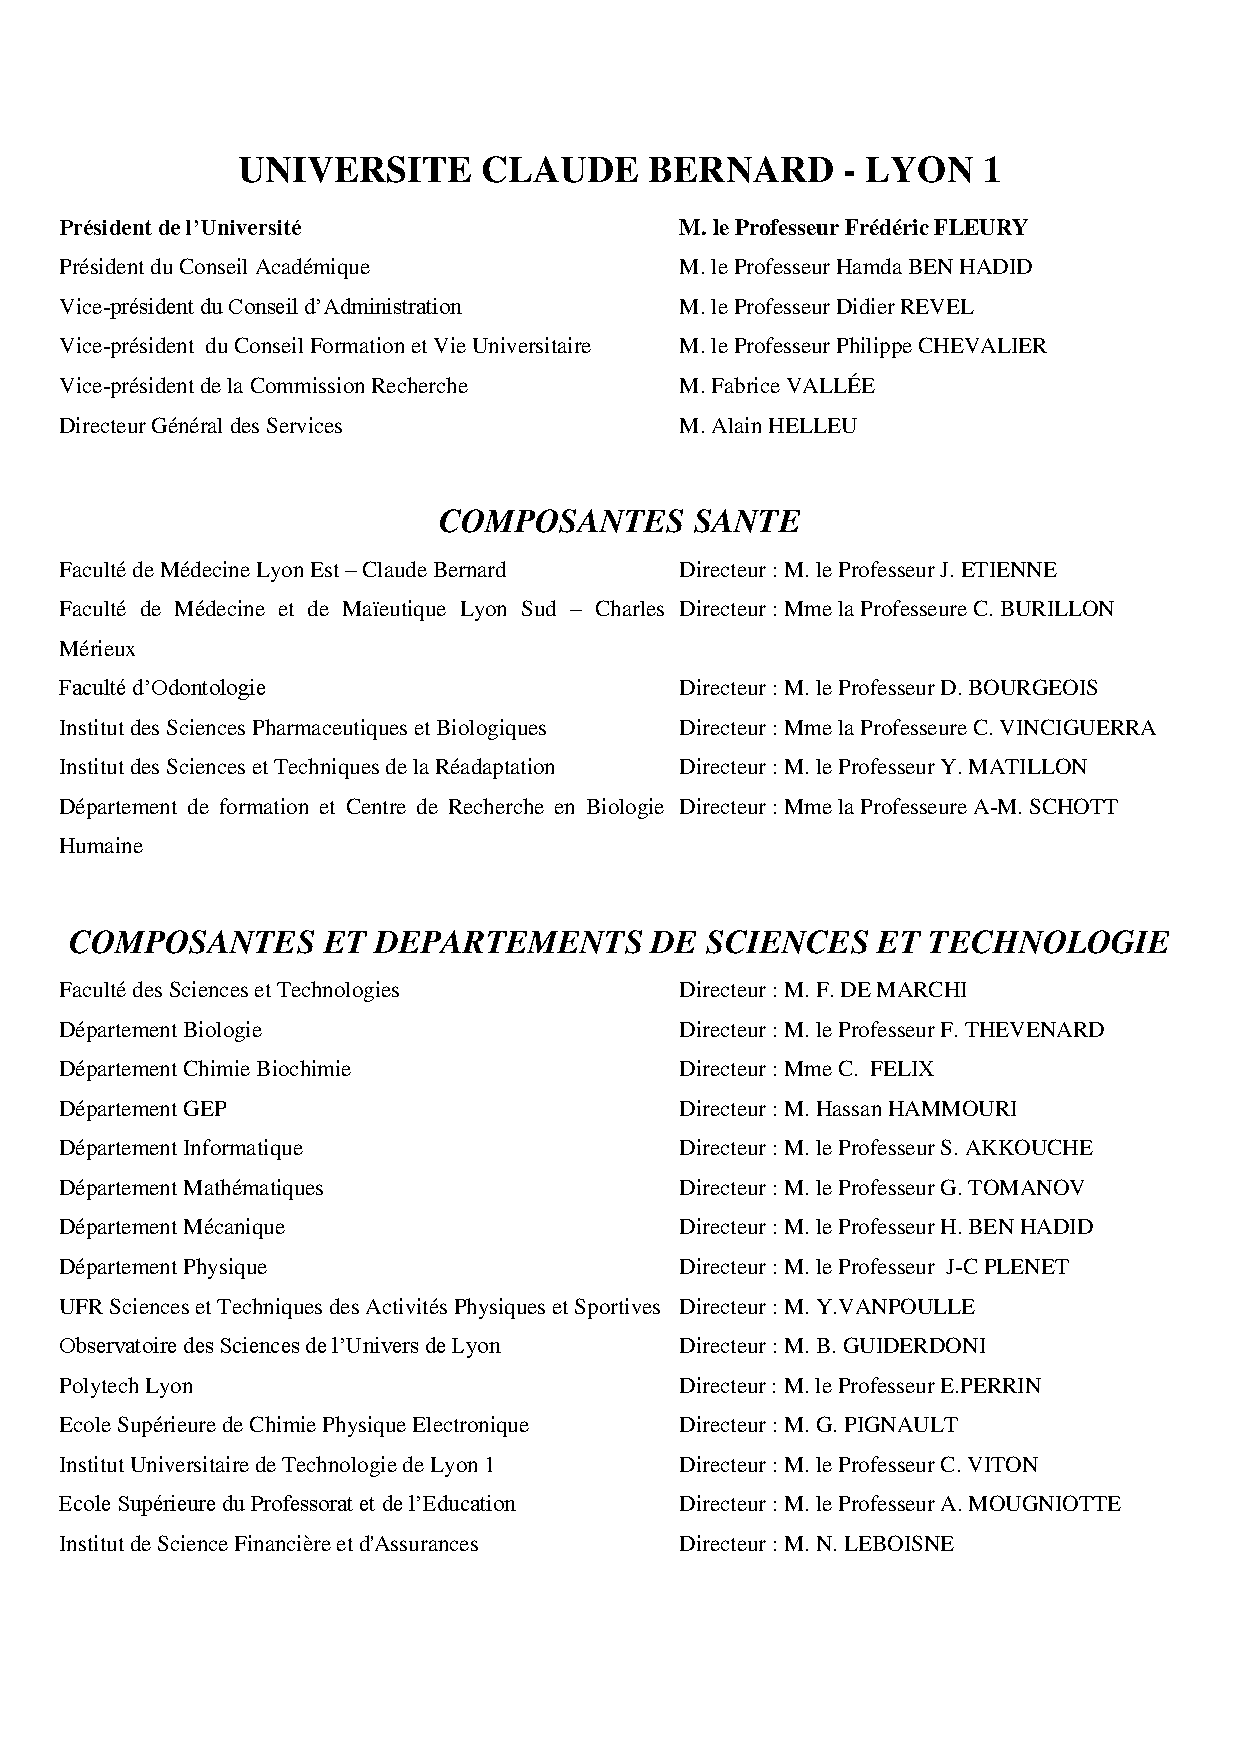
\includepdf[pages=-, fitpaper=true]{content/composante_lyon1.pdf}
\cleardoublepage

% 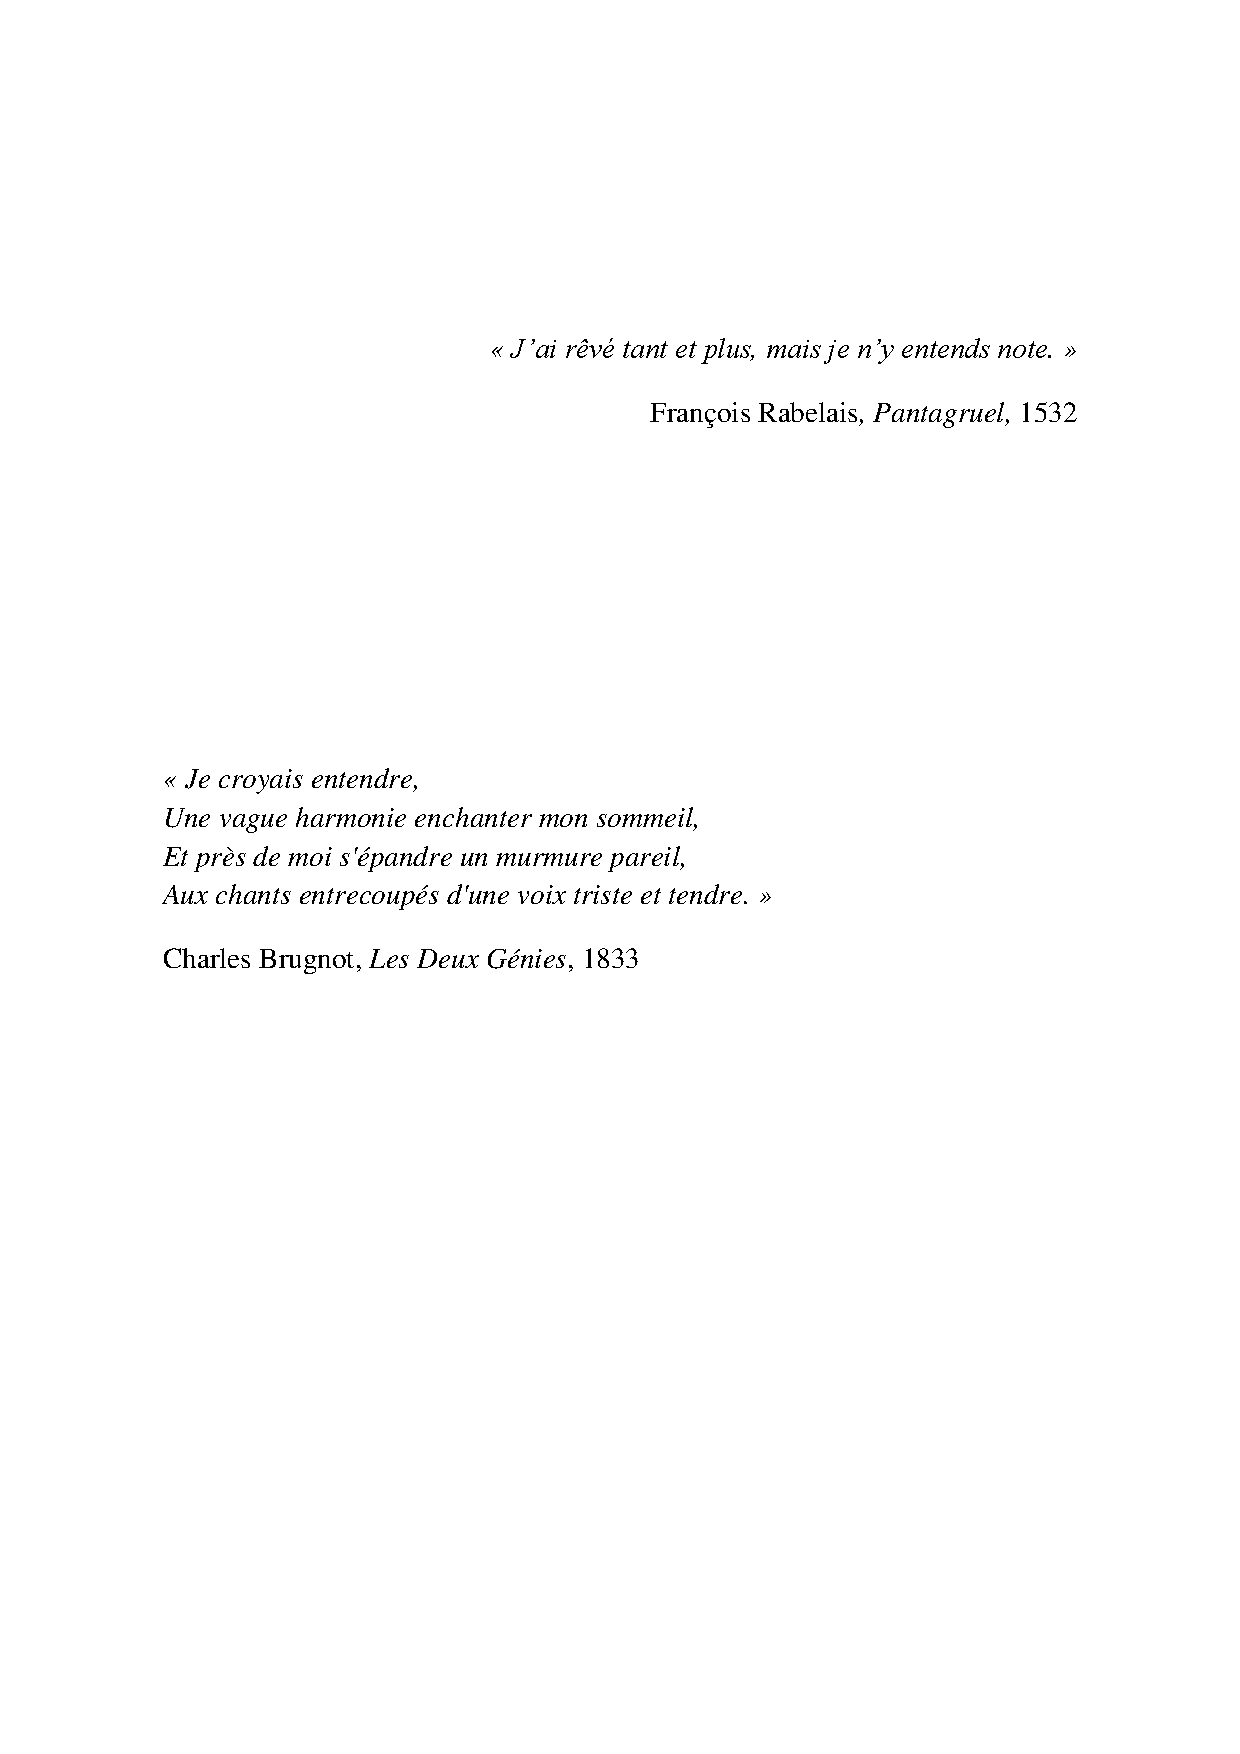
\includepdf[pages=-]{content/citation.pdf}
% \cleardoublepage

\pagestyle{plain}				% display just page numbers
% % !TEX root = ../thesis-example.tex
%
\pdfbookmark[0]{Abstract}{Abstract}
\chapter*{Abstract}
\label{sec:abstract}
\vspace*{-10mm}

\blindtext

\vspace*{20mm}

{\usekomafont{chapter}Résumé}\label{sec:abstract-diff} \\

\blindtext
		% INCLUDE: the abstracts (english and french)
% \cleardoublepage
% %
% % !TEX root = ../thesis-example.tex
%
\pdfbookmark[0]{Acknowledgement}{Acknowledgement}
\chapter*{Acknowledgement}
\label{sec:acknowledgement}
\vspace*{-10mm}

Je tiens avant toute chose à remercier Perrine Ruby, ma directrice de thèse, dont la confiance et le soutien ont rendu possible ce travail. Tu sais, je l'espère, toute la considération et l'amitié que j'ai pour toi, et je ne te remercierai jamais assez de m'avoir toujours poussé vers l'avant, par exemple en me permettant de faire de nombreux congrès (et cela avant même de commencer ma thèse !). Ta rigueur et ton honnêteté scientifique, ainsi que ton engagement constant et indéfectible pour tes étudiants, sont tout autant de qualités que je souhaiterai avoir s'il m'est permis un jour d'encadrer des étudiants.

Ma pensée se tourne ensuite vers tous les membres du laboratoire DYCOG avec qui j’ai vécu et partagé des moments inoubliables tout au long de ces quatre dernières années. Sans pouvoir citer, par soucis écologique, toutes les personnes avec qui j’ai échangé, je tiens tout de même à évoquer mes collègues et amis du bureau d’en haut, Laurie-Anne, Kony, Etienne, Enrico, Stefano, dont la présence au Vinatier ne relève sans doute pas d’un hasard total ; les copains du café de 7 h et du saucisson de 19 h, Florian, Benoit, Thibault ; l’équipe des méditants Croix-roussien, Kristien, Antoine, Jelle, Oussama, pour ces moments de rire au milieu des fameux bouchons Lyonnais ; et bien sûr tous les autres doctorants, étudiants, ingénieurs, chercheurs, et personnels administratifs de ce laboratoire pour leur expertise scientifique et, surtout, leur bonne humeur qui rend la vie si agréable dans ce laboratoire.

Toute ma gratitude se porte également aux participants de nos expériences, d’imagerie ou de comportement, qui sont de fait la composante essentielle de ce travail. Ils nous ont prêté leurs rêves et leurs cerveaux, tout en gardant une motivation sans faille et un sourire constant.

Je pense ensuite à mes amis proches, Ylane, Caroline, Olivier, Géraud, Alex, Matthieu, Bertrand, qui ont su égayer ma vie durant toutes ces années, à coup de rires, de délires et de musique.

Le meilleur pour la fin dit-on - je remercie du fond du cœur mes parents, Isabelle et Alain ainsi que ma sœur Amélie et sa petite famille grandissante, sans qui tout cela n'aurait jamais été possible. Ma pensée finale se tournera vers Alisé, qui en plus d’être un sujet idéal pour étudier le sommeil au quotidien, est la personne avec qui je souhaite construire mes rêves.
 % INCLUDE: acknowledgement
% \cleardoublepage
%
\setcounter{tocdepth}{1}		% define depth of toc
\tableofcontents				% display table of contents
\cleardoublepage

% --------------------------
% Body matter
% --------------------------
\pagenumbering{arabic}						% arabic page numbering
\setcounter{page}{1}						% set page counter
\pagestyle{maincontentstyle} 				% fancy header and footer

% 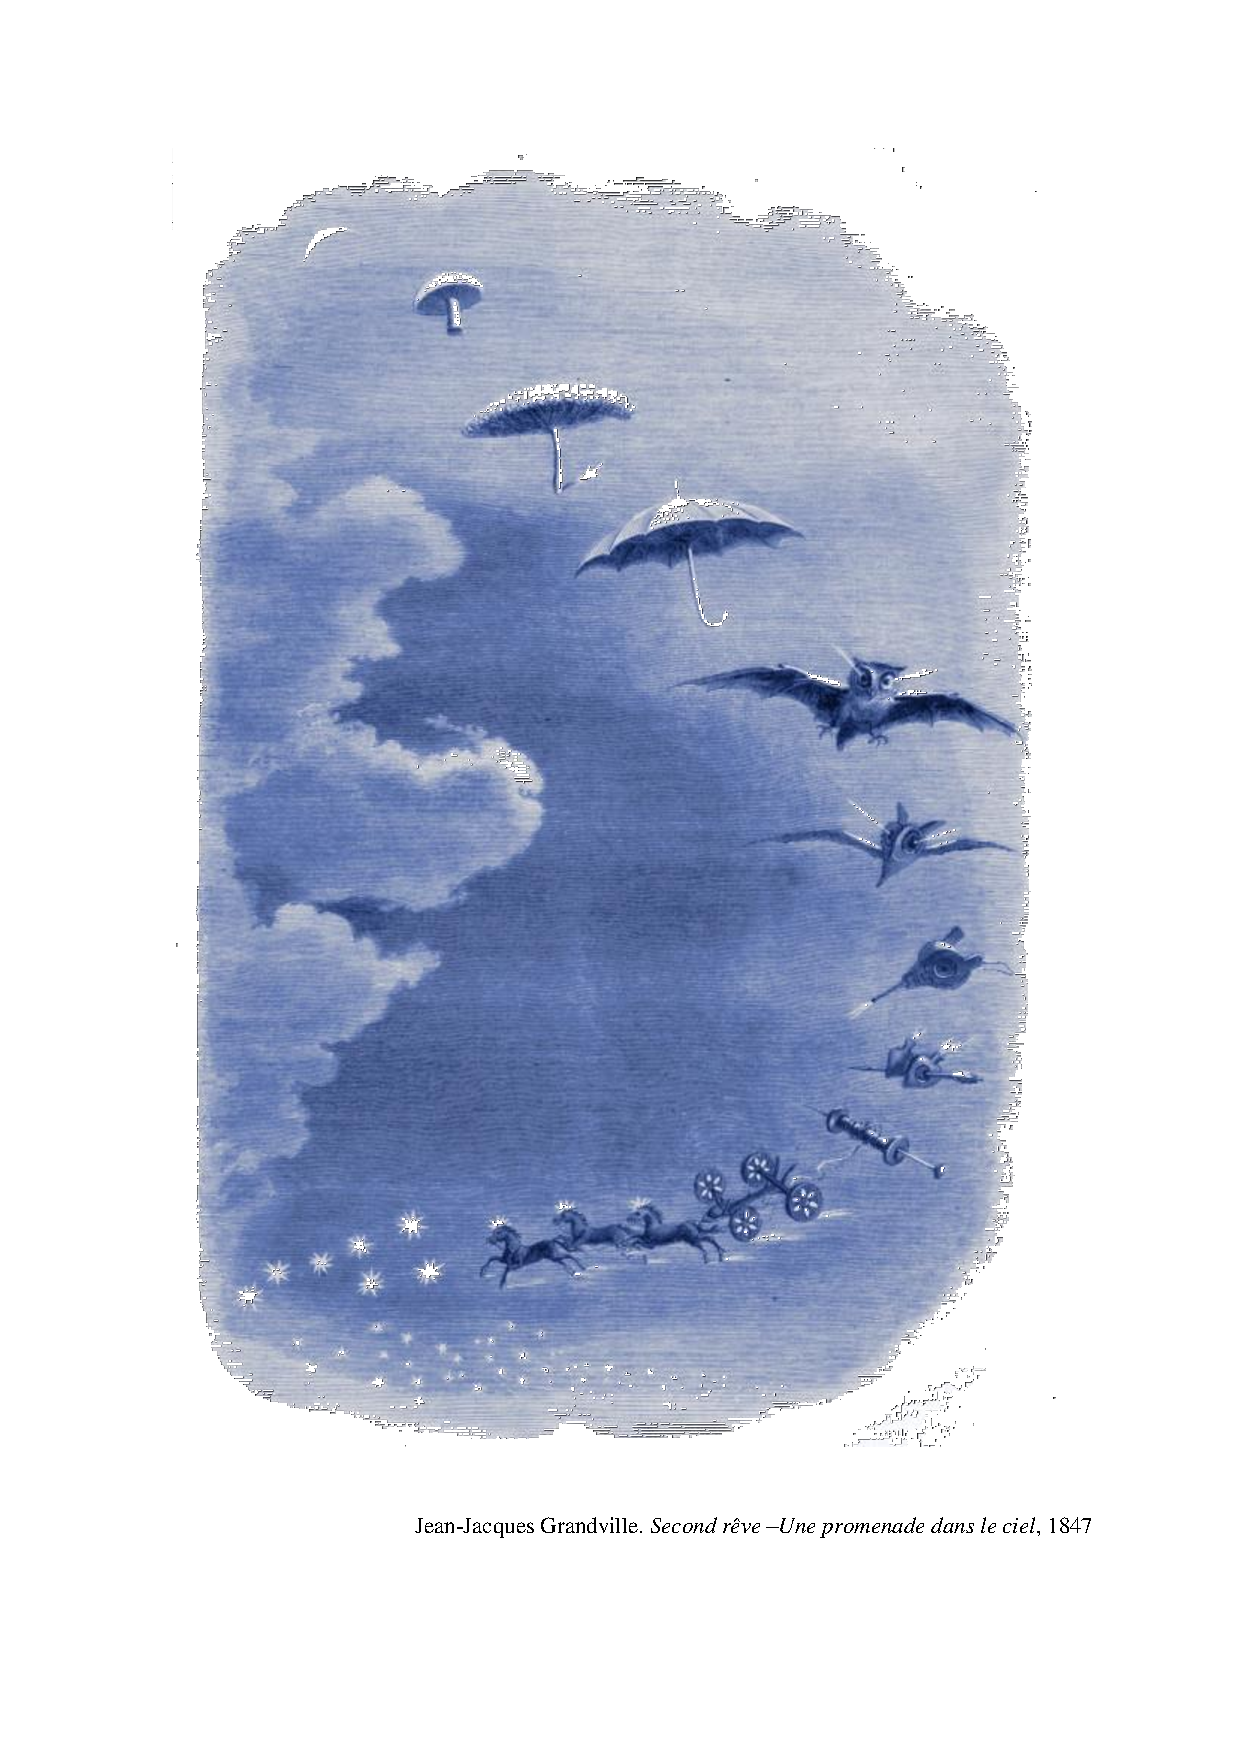
\includepdf[pages=-, pagecommand={\thispagestyle{plain}}]{content/grandville.pdf}
% \cleardoublepage

\part{GENERAL INTRODUCTION}
% !TEX root = ../thesis-example.tex
%
\chapter{Methods and problems in dream research}
\label{sec:dream-research}

\cleanchapterquote{Dream science holds an intermediate position between history and biology. It is a science of observation, because observation is an essential part of it, but it is also an historical science in the sense that the elapsed dream can never be reenacted and is therefore investigated, not directly, but through memory.}{Yves Delage}{Le rêve. Etude psychologique, philosophique et littéraire. 1920}

\section{Dreams}
\label{sec:dream-research:dreams}

\subsection{Definition}
\label{sec:dream-research:dreams:definition}

According to the Cambridge Dictionary, a dream is a \q{series of events or images that happen in the mind when one is sleeping}. This vague definition illustrates quite clearly how little we know about dreams, despite more than a century of experimental research and millennia of religious and philosophical speculation on their nature and meaning. The main reason for this lack of a clear and consensual definition (\cite{pagel_definitions_2001}) is that dreaming is \q{a phenomenon that we can solely observe during its absence} (Paul Valery, Analecta, 1926).  Indeed, we still do not know precisely when dreaming occurs during sleep, and the dreamer alone is witness to his or her dream. For that reason, the scientific study of dreaming relies critically on the introspective recall of the dreamer, or \q{retrospection} \citep{schwartz_dreaming:_2005}.

\subsection{Scientific perspective}
\label{sec:dream-research:dreams:science}

Therefore, a more scientific definition of dreaming was proposed by \citet{guenole_a_2009} who wrote that \q{dreaming is a mental experience during sleep, which can be remembered and reported at wake}. He further distinguished three successive and intertwined forms of the dreaming phenomenon. The primordial state is the dream-experience that happens during sleep, and of which very little is known because the dreamer has no means to communicate in real-time his or her oneiric experiences to the external world. With the notable exception of lucid dreaming, the dream-experience is unobservable to the waking consciousness, be it that of an external observer, but also that of the dreamer him- or herself. The second form is the memory of the dream-experience as we recall it after awakening. Importantly, the dream recall occur in a consciousness state different from the one in which the dream was experienced. As a memory object, dream recall is therefore likely to be influenced by several mechanisms such as forgetting, reconstruction, verbal description difficulties and censorships (\cite{schwartz_sleep_2002, schwartz_dreaming:_2005}). The third and last form is the dream report, obtained after transcription of the dream recall using words or pictures. The dream report is the only one that can actually be communicated to others and therefore the only one eligible to empirical investigation. As a consequence, most of the dream research has focused on dream reports.

\begin{figure}[htb]
	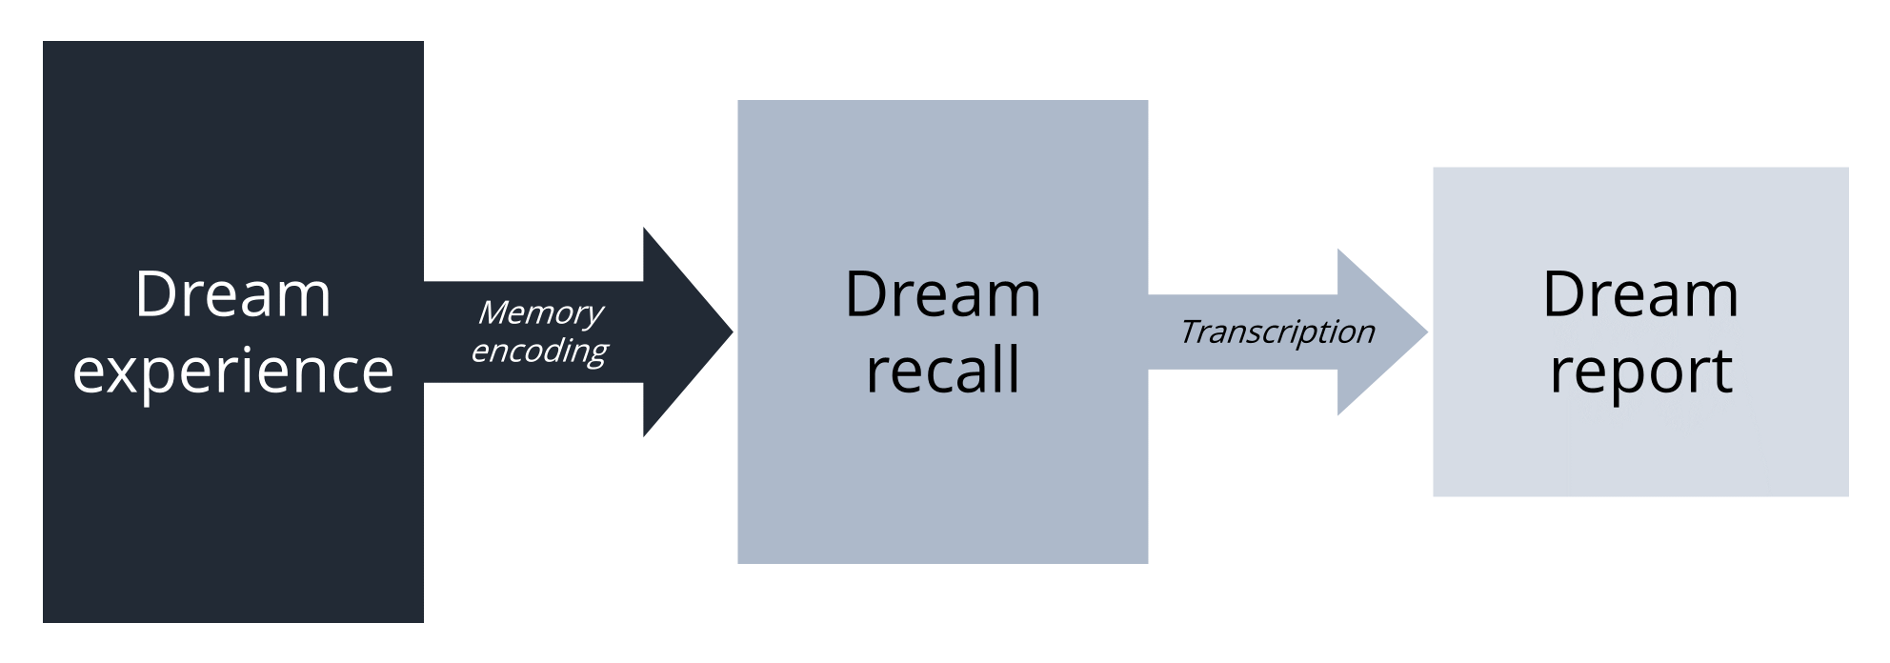
\includegraphics[width=\textwidth]{Fig/Intro/Intro_Guenole/Intro_Guenole.png}
	\caption[Guénolé's model of dreaming]{Guénolé's model of dreaming}
	\label{fig:intro:guenole}
\end{figure}

Because of this elusiveness of dreams and the constraints inherent to the scientific study of dreaming, it still remains one of the great mystery of the human cognition. Several questions on its nature and meaning are still not answered: do we dream every night? For how long? Why do we sometimes recall our dreams and sometimes not? Do dream reports obtained after awakening accurately convey subjective sleep experiences? What is, or what are, the function(s) of dreaming? What are the neurophysiological correlates of dreaming? The aim of the present thesis is to offer a modest contribution to the ongoing effort to solve these questions.

\section{Sleep}
\label{sec:dream-research:sleep}

As Schopenhauer rightly noticed, \q{the characteristic of dream is the condition of sleep peculiar to it}. Therefore, we cannot go any further in our study of dreaming without first defining the sleeping state and its physiology. Sleep is a normal physiological and periodic state characterized by vigilance suspension, which generally occurs during night time in humans. Sleep is a vital need that allows restoration of the immune, nervous, skeletal and muscular systems, leading some authors to postulate that \q{sleep is the price we pay for being alive} \citep{tononi_sleep_2014}. Long regarded as an idle state, it is becoming increasingly evident that sleep is \q{first and foremost a brain process} \citep{hirshkowitz_normal_2004} in which the brain is \q{hard at work and helps makes something of the world}, to borrow the words of Heraclitus’s famous aphorism (for an exhaustive review of the cognitive processes occurring during sleep, \citealt[see][]{andrillon_sleeping_2016}).

\subsection{Sleep stages}
\label{sec:dream-research:sleep:stages}

The invention of electro-encephalography (EEG) by Hans Berger in 1928 has paved the way for the scientific study of sleep. It was indeed soon after that discovery that Alfred Loomis first described a global slowing down of the brain rhythm during sleep, associated with the apparition of several grapho-elements such as K-complexes. Since then, sleep researchers have used EEG to monitor brain waves, electrooculography (EOG) to monitor eye movements and electromyography (EMG) to measure skeletal muscle activity. The simultaneous collection of these measurements is called polysomnography (PSG) and provides sufficient information to identify sleep stages according to standard international established guidelines. PSG is the gold standard in modern sleep science and is used in both clinical and research settings.

A first set of rules were published by Rechtschaffen and Kales (R\&K) in \citeyear{kales_manual_1968} and proposed to divide sleep into 5 stages with distinct electrophysiological properties, named rapid-eye movement (REM) and non-REM (NREM) stages 1, 2, 3, 4. This nomenclature was updated in 2007 by the American Academy of Sleep Medicine \citep{iber_aasm_2007} and sleep stage 3 and 4 have been merged into stage N3. Below are summarized EEG-EOG-EMG characteristics for wakefulness and the different sleep stages (see also Figure \ref{fig:intro:sleep_stage}).

\paragraph{Wakefulness}
Before diving into sleep, we first need to define the state of wakefulness. Eyes-closed quiet wakefulness is accompanied by an EEG rhythm predominantly in the alpha range (8-12 Hz). Opening the eyes or engaging in a significant mental task (for example mental calculation) reduces or blocks the alpha activity. Fairly high muscle activity can be present and slow or rapid eye movements may occur.

\paragraph{N1 sleep}
Stage N1 corresponds to the transitional period between wakefulness and sleep. The brain rhythm progressively decreases from alpha to theta (5 – 7 Hz), and the EOG is characterized by slow, rolling eye movements. N1 sleep represents approximatively 5\% of a normal night of sleep.

\paragraph{N2 sleep}
Each night, we spend more than half the night’s sleep in N2 sleep. The EEG activity during this stage is characterized by a predominance of theta waves, recurrently interrupted by two grapho-elements, the spindles and K-complexes, which are the landmarks of this sleep stage. K-complexes are defined as sharp negative waves followed by a positive component, prominent over frontal scalp electrodes and lasting more than 0.5 seconds. Spindles refer to burst of 12 to 14 Hz waves predominant over central scalp electrodes and lasting between 0.5 and 2 seconds. Beyond that, N2 sleep is characterized by an absence of eye movements as well as decreased muscle tone and brain metabolism.

\paragraph{N3 sleep}
N3 sleep, also referred to as deep sleep or slow-wave sleep, is the deepest sleep stage. It is characterized by a predominance (> 20\% of the epoch) of high amplitude (> 75 µV) delta waves (0.5 – 4 Hz). Eye motility, muscle tone and brain metabolism are even more decreased than in N2 sleep. N3 sleep represents approximatively 20\% of a normal night of sleep.

\paragraph{REM sleep}
As its name suggests, rapid eye movements (REM) sleep is characterized by rapid eye movements easily observable on the EOG channels. They consist of conjugate, irregular and sharply peaked eye movements, similar to some extent to those exhibited during wakefulness. Another fundamental aspect of REM sleep is its muscle atonia, as revealed by a low EMG activity. However, some transient muscle activity or muscle twitching (MTs) can also be observed. These short irregular bursts of EMG activity are superimposed on the background of low EMG activity. Brain metabolism is similar to that of wakefulness, and the EEG is marked by mixed low-amplitude waves predominantly in the theta band (saw-tooth waves), as well as a complete absence of delta rhythms. Other physiologic activities accompany REM sleep including middle ear muscle activity, periorbital integrated potentials, and sleep-related erections. REM sleep constitutes approximatively 20\% of a normal night of sleep.

\begin{figure}[htb]
	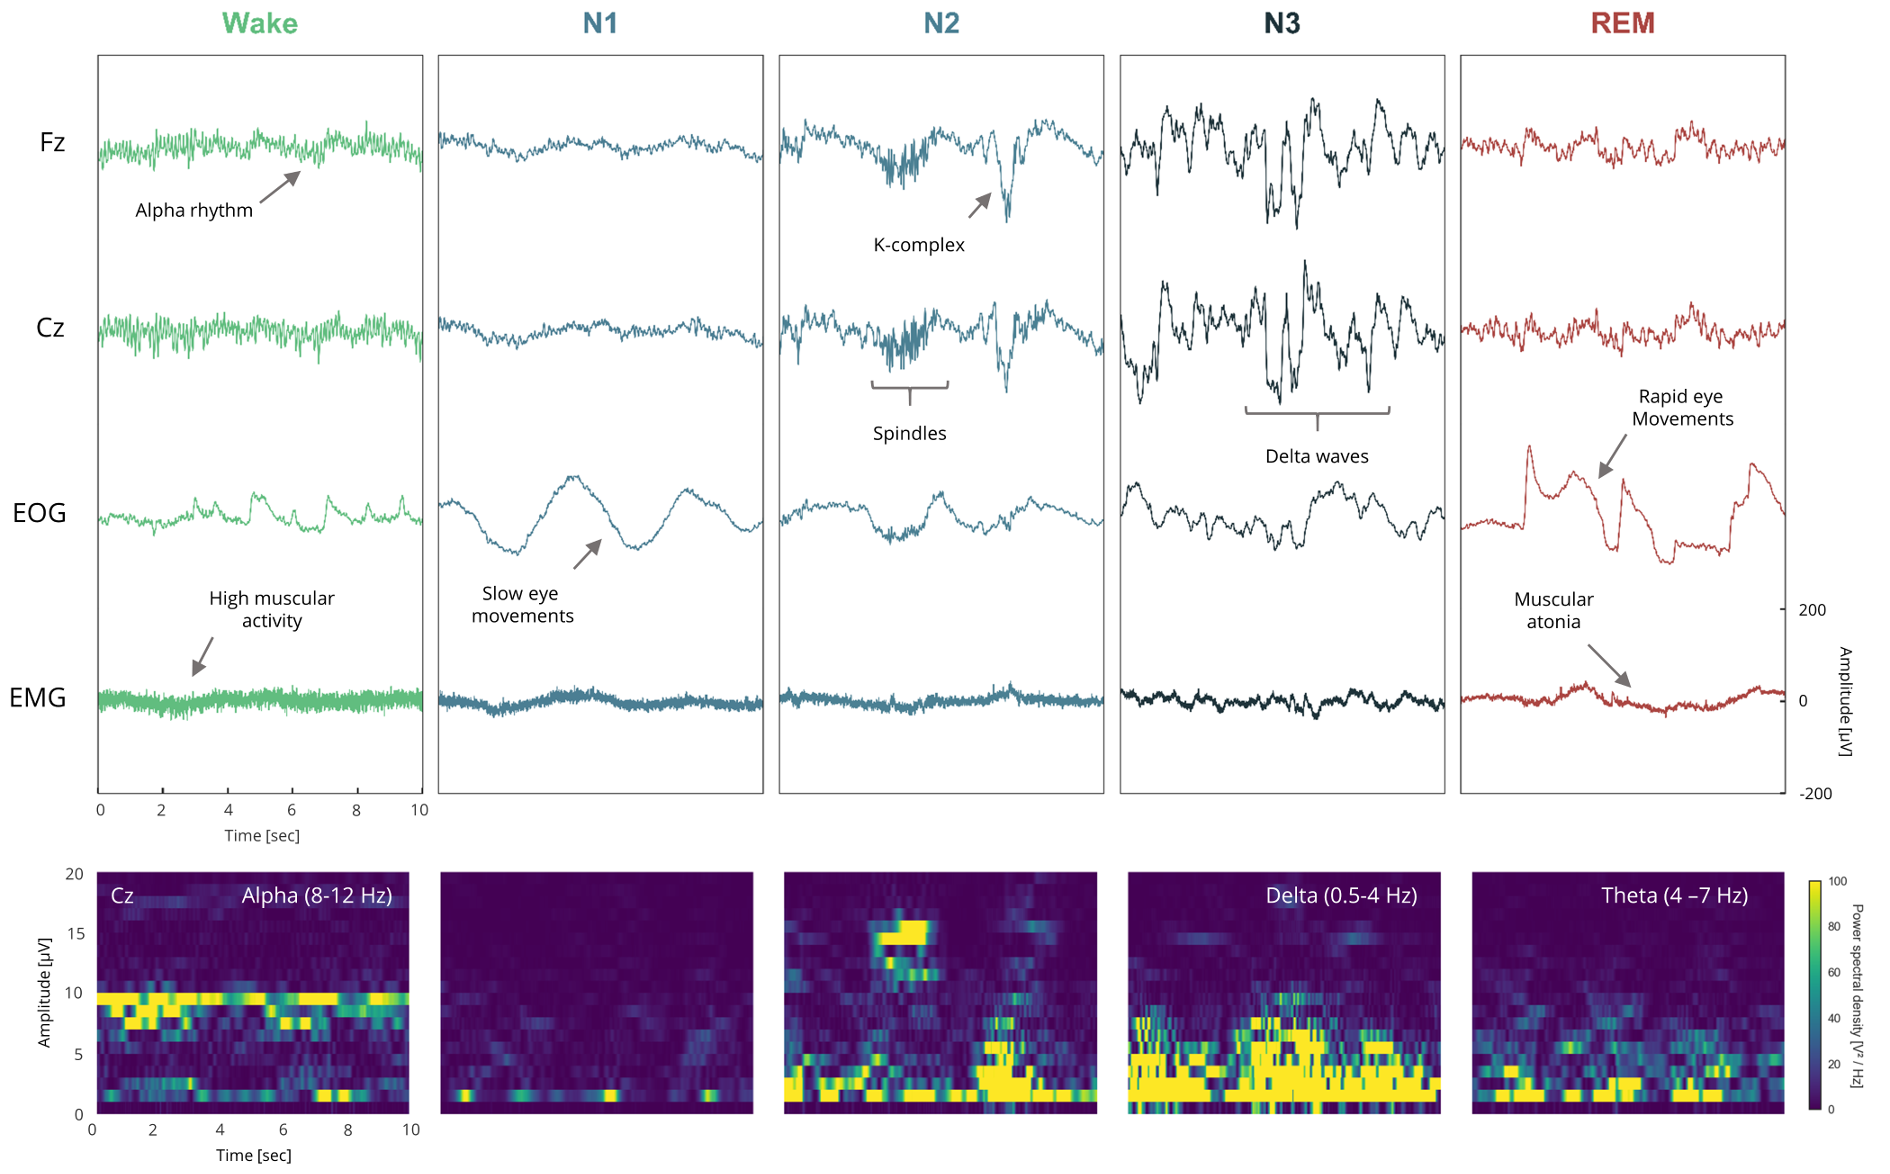
\includegraphics[width=\textwidth]{Fig/Intro/Intro_Sleep_Stages_PSD/Fig_Intro_Sleep_Stages_PSD_final_150517.png}
	\caption[Polysomnographic recordings across sleep and wakefulness]{Polysomnographic recordings across sleep and wakefulness. Top: Scalp EEG, EOG and EMG performed in one healthy young adult during wakefulness, N1, N2, N3 and REM sleep. The main features of each vigilance state are described. Bottom: Spectral properties of each stage obtained by computing the spectrogram of the Cz EEG signal atop.}
	\label{fig:intro:sleep_stage}
\end{figure}

\subsection{Sleep architecture}
\label{sec:dream-research:sleep:architecture}

Modern research has revealed that sleep is not a unitary, single block, but rather a cyclical succession of different brain states, which are all associated with specific functional roles. A normal night of sleep consists of a repetition of four or five 90 to 110 minutes long cycles in which sleep stages tend to follow each other in a particular order. The sleep cycle properties evolve with each cycle reoccurrence. Sleep staging is generally done visually by inspecting consecutive polysomnographic segments of 30 seconds. It results in a hypnogram which represents the succession of sleep stages across time (Figure 3). In his overview of the human sleep, Hirshkowitz described five generalizations about normal sleep architecture \citep{hirshkowitz_normal_2004}:

\begin{my_list_num}
    \item Sleep is entered through non-REM sleep
    \item Non-REM and REM sleep alternate approximately every 90 to 120 minutes
	\item N3 sleep predominates in the first third of the night
	\item REM sleep predominates in the last half of the night
	\item REM sleep occurs in four to six discrete episodes each night with episodes generally lengthening as sleep period progresses
\end{my_list_num}

\begin{figure}[htb]
	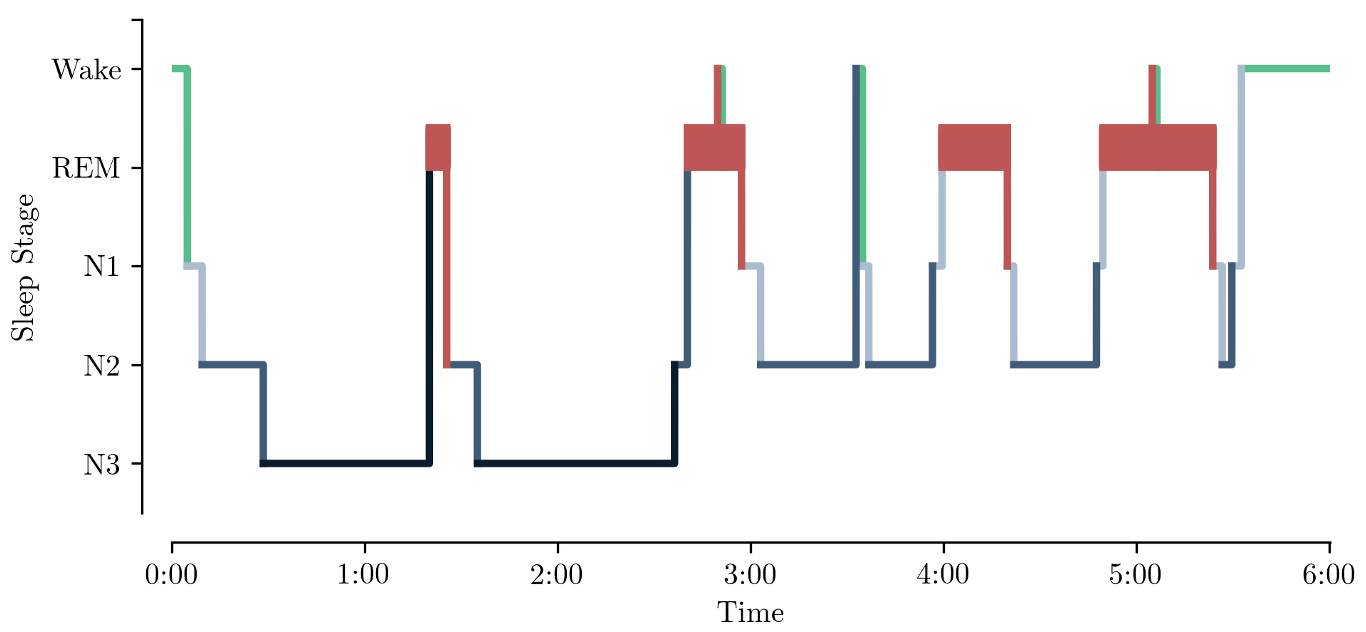
\includegraphics[width=\textwidth]{Fig/Intro/Intro_Hypnogram/Intro_Hypnogram.png}
	\caption[Example hypnogram of a healthy adult]{Example hypnogram of a healthy adult. The hypnogram is a graph which represents the stages of sleep as a function of time.One can easily recognize the succession of sleep cycles and especially the alternance of NREM (blue gradient) and REM sleep (red). Note that the hypnogram graph was generated directly as it is from the sleep software presented in the experimental results section.}
	\label{fig:intro:hypno}
\end{figure}

\section{Link between dreaming and sleep stages}
\label{sec:dream-research:link}

\subsection{The REM sleep hypothesis of dreaming}
\label{sec:dream-research:link:rem-sleep}

In the early fifties, Nathaniel Kleitman and his doctoral student Eugene Aserinsky, discovered in humans the existence of periods of sleep with an EEG similar to wakefulness (low voltage and fast frequencies), rapid eye movements and neurovegetative responses \citep{aserinsky_regularly_1953}. This discovery had a strong and persistent impact on dream and sleep research. The authors have indeed proposed that the rapid eye movements corresponded to the scanning of dream images. They reached this conclusion by comparing the proportion of dream reports obtained upon awakening in periods of eye motility and outside these periods, respectively 75\% and 11\% in their 1953’s study, and 80\% and 7\% in their 1957's study \citep{dement_relation_1957}. They concluded that their newly-discovered REM sleep stage was the neurophysiological basis of dreaming. A few years later, the French neurophysiologist Michel Jouvet, who had started working on sleep in cats, found that REM sleep was associated with muscular atonia \citep{jouvet_sur_1959}, a finding that was soon after replicated in humans \citep{berger_tonus_1961}. Pursuing his research on REM sleep, or \q{paradoxical sleep} as he named it, Jouvet had the idea to suppress the muscular atonia by injuring the brain stem of cats. To his astonishment, he found that the injured cats were performing, only during REM sleep, complex motor sequences, that he named \q{oneiric behavior} \citep{sastre_comportement_1979}. For him and the scientific community at the time, it was clear that these motors sequences were directly related to the cat's dreams, and this experiment provided a significant evidence in favor of the REM sleep hypothesis of dreaming.

However, even though equating dreaming with REM sleep provided a useful way to scientifically explore dreaming, it soon became apparent that dreaming was in fact not exclusively present during REM sleep but also during all the other sleep stages. Few years after the initial discovery of REM sleep, several researchers reported a much higher proportion of dream report in non-REM sleep than what was expected based on the findings of the Kleitman’s team \citep{goodenough_comparison_1959, foulkes_dream_1962}. Comparing the recall rate of people who never remembered their dreams with people who frequently recalled them, Goodenough and colleagues found respectively 34\% and 54\% of dream reports outside of REM sleep. The recall rate went up to 54\% in Foulkes’s study which comprised 200 awakenings. Since then, numerous studies have replicated the finding of mentation outside of REM sleep \citep{nielsen_review_2000}, even in the periods of non-REM sleep located before the first nocturnal episode of REM sleep \citep{noreika_early-night_2009}. As a counterpoint, it has become apparent that a significant proportion (~15\%) of REM sleep awakenings were not followed by a dream report. It results that dreaming is not specific of REM sleep.

Despite the REM sleep hypothesis of dreaming is still present in the public mind, the occurrence of dream mentation in all sleep stages is increasingly accepted in the scientific community. As Schwartz and colleagues aptly pointed out, \q{REM sleep is not a necessary, but a facilitating condition for dreaming to occur. Conversely, there is little doubt that dreaming was a necessary condition for REM sleep to become famous} \citep{schwartz_dreaming:_2005}.

\subsection{The fore-brain hypothesis of dreaming}
\label{sec:dream-research:link:solms}

Equating dreaming with REM sleep, Hobson argued that dreaming depends on the brainstem REM sleep generator \citep{hobson_dream_1998}. This was the dominant theory for several decades until a firm opponent of the REM sleep hypothesis of dreaming, Mark Solms, refuted it using neuropsychological evidences. He examined 361 neurological patients and asked them in detail about their dreaming \cite{solms_neuropsychology_1997}. He found that out of 26 case reports of REM sleep loss or alteration following a lesion in the brainstem (Pons area), 25 were not associated with subsequent alterations in dream reporting. By contrast, he reported that in most cases global cessation of dreaming (a condition referred to as the Charcot-Wilbrand syndrome) followed lesions in or near the temporo-parietal junction (TPJ) and the medial prefrontal cortex (MPFC; see Figure \ref{fig:intro:lesions}). Importantly, damage in these two regions were rarely associated with REM sleep disturbances. This double dissociation provides a clear argument that not only dreaming can occur outside of REM sleep, but it is also not dependent of the brainstem generators of REM sleep. This led Solms to put forward the fore-brain hypothesis of dreaming, which proposes that dreaming is controlled through forebrain mechanisms involving at least TPJ and MPFC.

\begin{figure}[htb]
	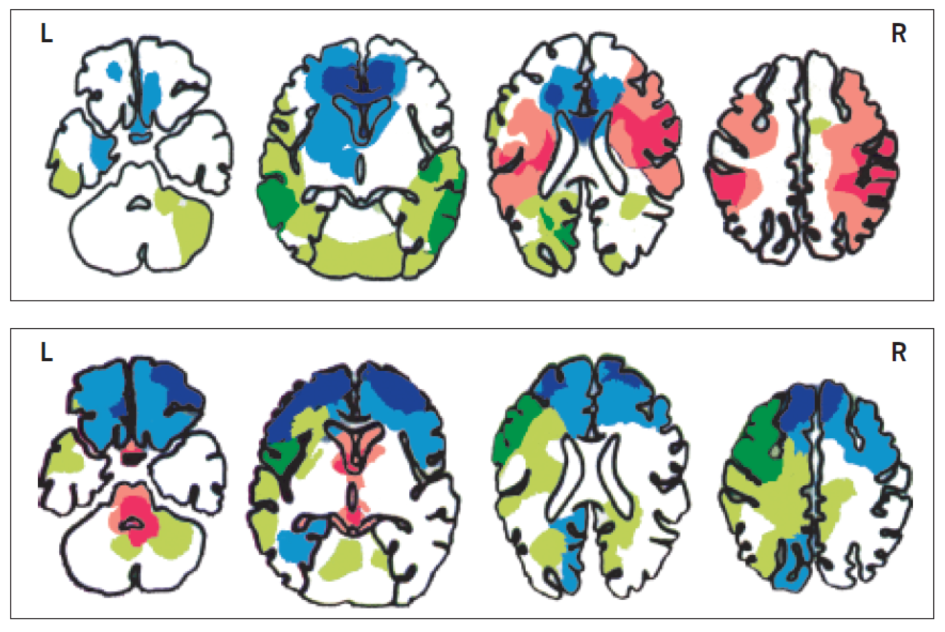
\includegraphics[width=\textwidth]{Fig/Intro/Intro_Lesions/Intro_Lesions.png}
	\caption[Lesion maps associated with cessation vs preservation of dreaming]{Lesion maps associated with cessation vs preservation of dreaming. Top: Global cessation of dreaming was found following parietal lobe lesions (6 cases, inferior lobule and supramarginal gyrus; red), medial frontal lesions (9 cases; blue), and posterior lesions (8 cases; green). Bottom: Preserved dreaming was found following left hemispheric and frontal convexity lesions (15 cases; green), bifrontal lesions (14 cases; blue), and brainstem lesions (17 cases; red). Reproduced from \citet{schwartz_dreaming:_2005}}
	\label{fig:intro:lesions}
\end{figure}

\subsection{A continuum of mentation during sleep}
\label{sec:dream-research:link:continuum}

Based on Solms’s findings, some authors have postulated that instead of relying on REM sleep mechanisms, dreaming might be best described along a \q{continuum} of mentation during sleep, ranging from the hypnagogic reveries typical of sleep onset to florid and vivid dreamlike experiences typical during REM sleep \citep{schwartz_dreaming:_2005}. A brief description of this continuum of mental activities during sleep is reported in Table \ref{tab:intro:continuum}.

% Please add the following required packages to your document preamble:

\begin{table}[htb]
\caption[A continuum of sleep mentation]{A brief description of sleep mentation in their typical order of placement during the sleep cycle. Modified from \citet{de_koninck_sleep_2012}}
\label{tab:intro:continuum}
\resizebox{\textwidth}{!}{%
\begin{tabularx}{\textwidth}{XXX}
\toprule
\textbf{Name}                                                         & \textbf{Description}                                                                          & \textbf{Sleep stage}                         \\ \midrule
Hypnagogic reverie                                                    & Simple images                                                                                 & Sleep onset mentation (N1 or early N2 sleep) \\
Reflections                                                           & Thoughts with no hallucinatory content                                                        & N2 sleep                                     \\
Vivid dreams                                                          & Vivid imagery and sequences, presence of characters, interactions and emotions                & REM and NREM sleep                           \\
Lucid dreams                                                          & The dreamer is conscious of dreaming and can sometimes controls the dream scenario            & REM sleep                                    \\
Nightmares and bad dreams 	  										  & Unpleasant and highly anxiogenic dream. The content of nightmare actually awakens the dreamer & REM sleep                                    \\
Hypnopompic reverie                                                   & Characterized by elaborate imagery                                                            & Sleep offset mentation (REM or NREM sleep)   \\ \bottomrule
\end{tabularx}%
}
\end{table}


\section{Attempts to study the cerebral correlates of dreaming}
\label{sec:dream-research:attempts}

Thanks to the recent advances in neuroimaging techniques, we have the means to measure, with unprecedented spatial and temporal accuracy, what is happening in the brain at a specific moment in time (see Methods section). Yet, since it is now well-accepted that dreaming can occur in all sleep stages, and because dream consciousness is only accessible via report rather than direct observation, it is therefore impossible to be sure that dreaming is happening at a specific time point during sleep. This conceptual issue has not prevented sleep and dream researchers to attempt to identify the cerebral correlates of dreaming. The main methods and findings are summarized in the following paragraphs.

\subsection{Brain activity during REM sleep}
\label{sec:dream-research:attempts:ba-rem}

On the basis of the REM sleep hypothesis of dreaming, which was predominant during the nineties, researchers used functional neuroimaging techniques such as positron emission tomography (PET) to investigate the brain activity during REM sleep. They reported that, despite strong similarities between the wake and REM sleep electrophysiological scalp signals, the brain metabolism in these two vigilance states was disparate \citep{maquet_functional_1996, braun_regional_1997}. Among the most notable findings, the regional cerebral blood flow (rCBF) was decreased in several brain regions including the dorsolateral prefrontal cortex (DLPFC), and was increased in other regions (occipital, temporal, and superior parietal cortices, hippocampal formation, anterior cingulate and the pons). Following these works, researchers postulated that these changes in the brain functional organization could explain the phenomenological characteristics of dream reports \citep{hobson_dreaming_2000, nir_dreaming_2010}. For instance, increased occipital cortex activity during REM sleep could explain the clear predominance of visual modality in dream reports, a phenomenon that Vincent van Gogh had already noticed when he wrote: \q{I often think that the night is more alive and more richly colored than the day} (Vincent van Gogh, 1888). Second, the increased activity during REM sleep in the hippocampal formation, a region well-known for its role in memory encoding and retrieval, could account for the presence of known images and characters in dreams. Finally, the decreased activity in the dorsolateral prefrontal cortex, a region involved in executive function, cognitive control and working memory, could account for the lack of consistency, voluntary control and logical reasoning over the dream story. This is consistent with studies on lucid dreaming which showed a partial reactivation of this area in lucid dreams compared to non-lucid dreams. We will return to these correspondences between the phenomenology of dreams and brain activity in the chapter on the default mode network.

\subsection{Brain activity during lucid dreaming}
\label{sec:dream-research:attempts:ba-lucid}

Long considered as a fantasy, lucid dreaming - the ability to become self-aware of dreaming during a dream, and in some cases, to control the dream scenario – has recently gained considerable interest among researchers and the public. The scientific study of lucid dreaming started in the nineteenth century when Hervey de Saint Denys, a learned oneirologist, published his landmark book \q{Dreams and the Ways to Direct Them: Practical Observations}, in which he described his own lucid dream experiences. More than a century later, more objective methods such as EEG and functional magnetic resonance imaging (fMRI) have become the technique of choice for understanding lucid dreams. Using a pre-determined ocular signal, Dresler was remarkably able to measure, in real-time, the brain activity during lucid REM sleep and non-lucid REM sleep (though only one subject out of four had lucid dreams of sufficient length; \citet{dresler_neural_2012}). Lucid REM sleep was associated with a reactivation of areas that are normally deactivated during REM sleep, such as bilateral precuneous, parietal lobules and prefrontal and occipito-temporal cortices. Phenomenologically, these regions are either involved in self-awareness and executive functions, and their reactivation during lucid dreaming could account for the resurgence of a certain level of self-awareness and voluntary control. Even more recently, Voss was able to induce self-reflective awareness during dream using fronto-temporal transcranial alternating current stimulation \citep{voss_induction_2014}. They reported that lucid dreams were most prominent during stimulation in the lower gamma band (58\% of lucid dreams following a stimulation at 25 Hz and 77\% of lucid dreams following a stimulation at 40 Hz). However, the lucidity was not assessed directly by the dreamer but assumed a posteriori if the subjects reported elevated ratings on a lucidity scale. In conclusion, lucid dreaming provides an appealing and elegant way to study, in real time, the cerebral correlates of dreaming. Yet, the inherent problem with this method lies precisely in the fact that lucid dreams are, by nature, different from non-lucid dreams. As exciting as the results are, it would be however difficult to generalize them to the research on non-lucid dreams.

\subsection{Brain activity in the minutes preceding a dream report}
\label{sec:dream-research:attempts:ba-pre}

Another line of research consists in comparing the EEG power in various frequency bands in the minutes preceding a morning awakening associated, or not, with a dream recall. This paradigm has been used in several studies over the last decades, the findings of which are summarized as follows.

\citet{esposito_reduced_2004} reported that in both REM and N2 sleep, dream recall was associated with a lower alpha and delta power in the 3 minutes preceding awakening. According to the authors, the alpha effect may reflect increased cognitive elaboration and visual imagery as well as increased attention and memory processes. A few years later, \citet{marzano_recalling_2011} found that dream recall after morning awakening from REM sleep was associated with a higher frontal 5–7 Hz (theta) activity in the 5 minutes preceding awakening. In N2 sleep, dream recall was associated with a decrease in alpha power, an observation consistent with Esposito’s results. The same year, another study reported a lower delta power for the dream recall condition following awakening from N2 sleep, and a higher alpha and beta power in occipital derivations for REM sleep \citep{chellappa_cortical_2011}. Finally, a recent study, inaccurately entitled \q{the cerebral correlates of dreaming}, reported that in both N2 and REM sleep, reports of dream experience were associated with local decreases in delta power in posterior cortical regions in the 2 minutes preceding awakening \citep{siclari_neural_2017}. The authors were able to predict whether an individual reported dreaming or the absence of dream experiences after awakening from N2 sleep by monitoring this posterior ‘hot zone’ in real time.
The results from these studies are heterogeneous and sometimes contradictory. Moreover, despite this paradigm may seem attractive at first, the problem still remains that we can never be sure whether the dream actually took place in the minutes just before awakening or several tens of minutes before.

\subsection{Dreaming as a subsystem of the default mode network}
\label{sec:dream-research:attempts:dmn}

The past few years have witnessed the emergence of a new conceptual framework of dreaming, centered on the idea that dreaming is a unique form of mind-wandering, which cerebral correlates are a subsystem of the default mode network (DMN; see Methods section; \citealp{maquet_human_2005, domhoff_neural_2011, domhoff_dreaming_2015, christoff_mind-wandering_2016}). Based on the fact that dreaming and waking spontaneous thought share many features (i.e. predominance of the audiovisual modalities, centered on one’s current goals and concerns, draw heavily on semantic and episodic memory in constructing simulations and future plans, presence of a wide range of affect), some authors have postulated that dreaming is a \q{type of spontaneous thought that is highly unconstrained, hyper-associative and highly immersive} \citep{christoff_mind-wandering_2016}. Using the results of lesion and REM sleep neuroimaging studies, they argued that dreaming should be accompanied, at the neural level, by a strong recruitment of the default mode network medial temporal lobe (MTL)-centered subsystem and strong deactivations in frontoparietal control network regions (such as the DLPFC). Activation of the former areas could be related to the generation of spontaneous thoughts, during both wake and sleep, while the deactivation of the latter areas could explain the high volatility and variability of dream content over time.

\cleardoublepage
\cleardoublepage

\chapter{Dream recall frequency}
\label{sec:dream-recall}

\cleanchapterquote{We must also inquire what the dream is, and from what cause sleepers sometimes dream, and sometimes do not; or whether the truth is that sleepers always dream but do not always remember (their dream); and if this occurs, what its explanation is.}{Aristotle}{On dreams. 350 B.C.}

\section{Measuring dream recall frequency}
\label{sec:dream-recall:method}

As Aristotle had rightly pointed out, we do not always remember our dreams. More than two thousand years after, modern research has confirmed that the dream recall frequency (DRF) – i.e. the number of dream reports over a given period of time - is indeed highly variable both within individuals over the life course, but also between individuals \citep{schredl_factors_2003, ruby_experimental_2011}.

There is no gold standard for measuring DRF, and each method has its pros and cons. In research settings, three methods are commonly applied: questionnaire scales, dream diaries, and laboratory awakenings \citep{schredl_dream_1999}. The former consists in asking the participants to estimate their dream recall frequency over the last few weeks or months. This method has the advantage of being fast, inexpensive, and unaffected by the measurement, however, the DRF could be over- or under-estimated due to erroneous or incomplete recollection. Regarding dream diaries, the participants are asked to report each morning whether they have recalled a dream or not. This method minimizes the bias of retrospective estimation, but has the disadvantages of potentially increasing drastically the dream recall frequency, especially in persons who usually almost never recall their dreams \citep{schredl_questionnaires_2002}. Finally, laboratory awakenings consist in awakening the participants in the sleep lab and asking them whether they recall a dream or not. While this method has the clear advantage that the experimenters can measure physiological parameters (EEG, EOG, ECG, respiration and heart rate) prior, during and after the awakening, it is also time-consuming and expensive. Moreover, as for dream diaries, laboratory awakenings are associated with a dramatic increase in DRF, especially for low dream recallers.

\section{DRF in the general population}
\label{sec:dream-recall:pop}

\subsection{Average DRF}
\label{sec:dream-recall:pop:avg}

Measured by questionnaire, the average weekly DRF was 2.58 ± 2.03 in 444 German students \citep{schredl_factors_2003} and 0.83 ± 1.57 in a representative German sample of 931 participants \citep{schredl_dream_2008}. Using dream diaries, the average weekly DRF was 3.1 ± 1.5 in 70 Finnish children \citep{valli_threat_2005} and 3.9 ± 2.5 in a sample of 196 German student \citep{schredl_reliability_2005}. In lights of these results, we can conclude that the average weekly DRF in the general population lies between 1 and 3 dream reports per week.

\subsection{Intra-individuals variability}
\label{sec:dream-recall:pop:intra}

Daily experience suggest that our ability to recall dream fluctuate over time. Investigating this issue using the diary technique in 169 participants, \citet{schredl_reliability_2005} reported that the stability of DRF was very high over a period of one month. Similarly, he reported high DRF stability coefficients in a sample of older adults who had been interviewed weekly about their dream life over a period of 26 weeks \citep{schredl_reliability_2001}. However, to our knowledge, there are no studies evaluating the stability of DRF in the same individuals over an extended period of time.

\subsection{Inter-individuals variability}
\label{sec:dream-recall:pop:inter}

DRF varies drastically between individuals: some persons almost never recall a dream, whereas others can recall one or several dreams every morning. In an Austrian sample of 1000 persons, \citet{stepansky_austrian_1998} found that 31\% of the participants reported 10 dreams or more per month, 37\% reported between one and nine dreams per month, and 32\% reported less than one dream per month. In a sample of 285 German students, \citet{schredl_questionnaires_2002} found that 44\% reported dreams four or more times per weeks, 44\% reported a dream one time per week and 12\% reported a dream less than one time per month. This variability allows to differentiate behavioral profiles of DRF: high dream recallers (HR), who can recall a dream almost every morning (e.g. more than 5 mornings a week, \citealp{schredl_reliability_2005}) and low dream recallers (LR), who almost never recall a dream (e.g. less than one dream per month, \citealp{goodenough_comparison_1959}). Importantly, the frequency of HR is higher in the general population, and even more in young and/or student sample \citep{schredl_reliability_2005}.

\section{Parameters correlated with DRF}
\label{sec:dream-recall:param}

\subsection{Physiological and psychological factors}
\label{sec:dream-recall:param:psych}

First, increased professional or personal stress is positively associated with DRF \citep{schredl_dream_1999}. Similarly, an interest in dreams, or a positive attitude towards dreams is positively associated with DRF, as is frequent day-dreaming and rich fantasy life \citep{schredl_factors_2003}. DRF decreases with age and is slightly higher in women, who are also typically more interested in dreams \citep{schredl_dream_2008, schredl_gender_2008}. Regarding personality dimensions, studies have found positive correlations between DRF and thin boundaries, anxiety, and openness to experience \citep{hartmann_boundaries_1989, schredl_factors_2003,schredl_dream_2003}. However, most of the correlations between DRF and personality traits are low and explain only a small percentage of the total variance.

\subsection{Cognitive factors}
\label{sec:dream-recall:param:cogn}

Regarding cognitive abilities, a simple explanation of why individuals differ in their ability to remember dreams could be because they differ in some more general memory abilities (verbal, visual, short and long term). However, the literature yielded contradictory results, with some support for a positive association between DRF and visual memory, but also evidence against it for verbal and visual material and short-or long-term story narrative recall \citep{ruby_experimental_2011, blagrove_trait_2010}. On another note, several studies have consistently reported that DRF is positively correlated with creativity \citep{fitch_variations_1989, schredl_creativity_1995, schredl_factors_2003} and intelligence scales (multiple-choice vocabulary test, \citealp{schonbar_manifest_1959}, Shipley-Hartford intelligence scale, \citealp{connor_reported_1970}).

\subsection{Sleep parameters}
\label{sec:dream-recall:param:sleep}

First, DRF varies according to the sleep stage preceding awakening (see \citealp{nielsen_review_2000} for a review). More dream reports are obtained after an awakening during REM sleep than after an awakening during NREM sleep. These results inspired the REM sleep hypothesis of dreaming discussed earlier in section \ref{sec:dream-research:link:rem-sleep}. However, when a dream is not reported on awakening, there is no method of establishing whether it did not happen or was forgotten. This idea was rightly pointed out by \citet{conduit_poor_2004}: \q{An ongoing assumption made by sleep scientists is that since dreams are more often recalled on awakening from REM sleep, dreams must occur more often during this sleep stage. An alternative hypothesis is that cognition occurs throughout sleep, but the recall of mentation differs on awakenings}.

This idea that DRF variability is not a matter of dream production during sleep, but of dream recall during awakening, is the core of several models of dream recall (detailed later in section \ref{sec:dream-recall:theories}), among which the arousal-retrieval model is one of the most significant. In its simplest form, it claims that a period of wakefulness must occur just after dreaming so that the dream content can be transferred from short term to long term memory \citep{koulack_dream_1976}
Several studies support this model. First, using retrospective evaluation, \citet{schredl_factors_2003} found a positive correlation between the number of nocturnal awakenings and DRF. Second, \citet{de_gennaro_recovery_2010} reported that recovery sleep following a full night of sleep deprivation was characterized by an almost complete abolition of dream recall, paralleled with a lower number of nocturnal awakenings, which could, according to them, have \q{reduced the contents available in memory as possible cues for retrieval of dream experiences at morning}. Finally, these results were recently reinforced by a full-night PSG study in 36 subjects (18 HR and 18 LR; \citealp{eichenlaub_brain_2014}; Figure \ref{fig:intro:jbe-sleep}). HR showed in average longer intra-sleep wakefulness than LR (30 min vs 15 on average). The number of awakenings (the number of phases composed of consecutive pages of awakening) was not significantly different between the 2 groups, but the mean duration of the awakenings was (HR, 1.90 ± 0.91 min; LR, 0.95 ± 0.40 min).

\begin{figure}[htb]
	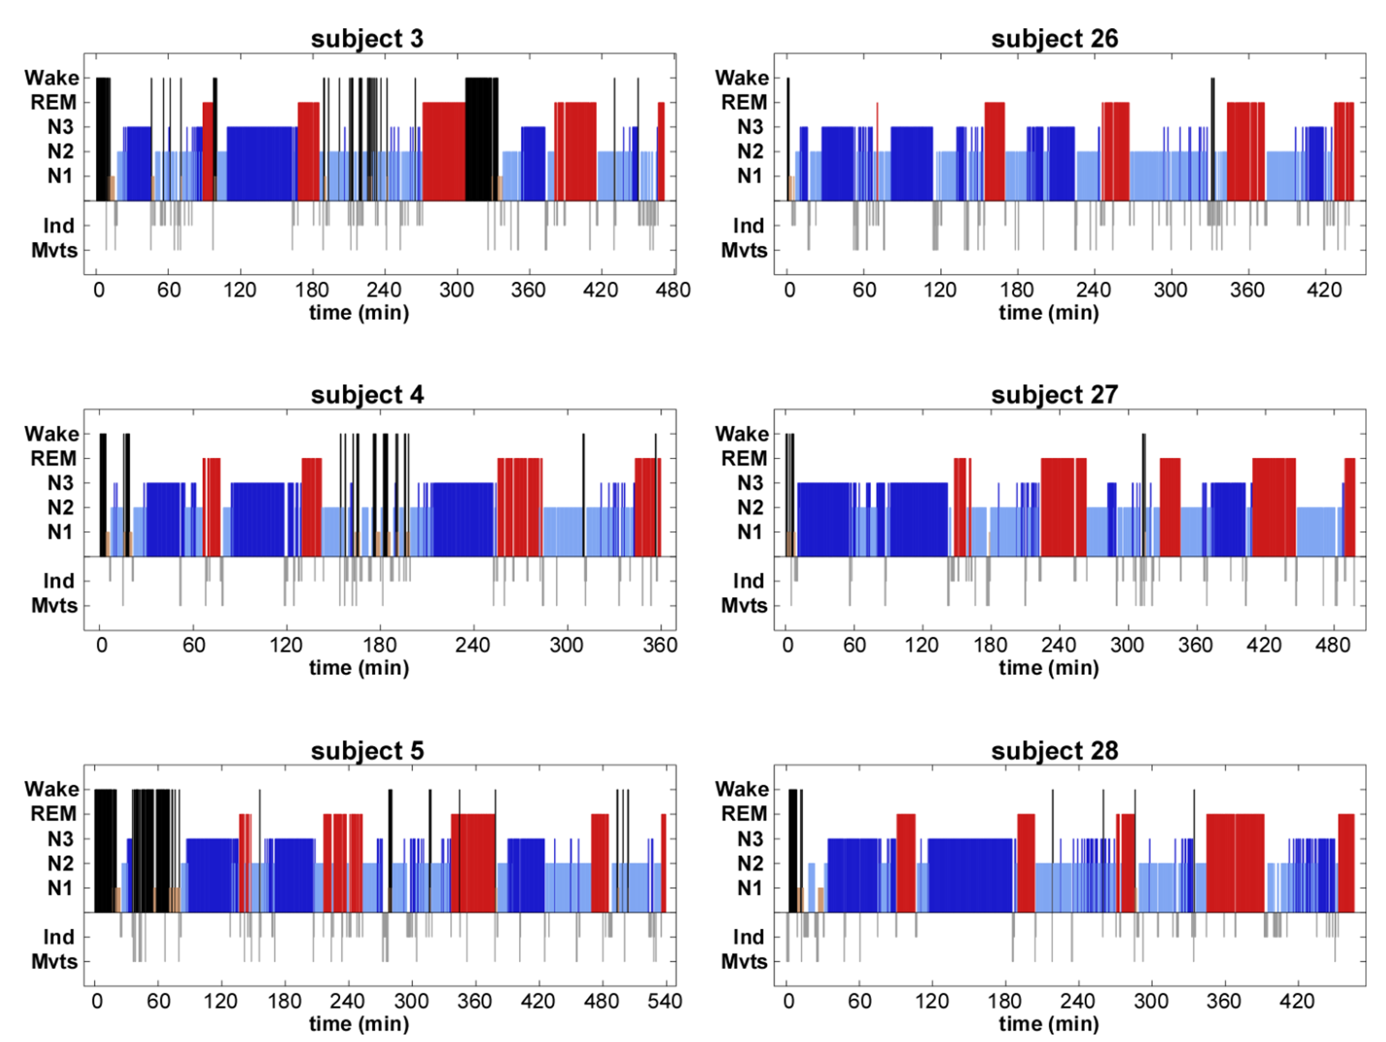
\includegraphics[width=\textwidth]{Fig/Intro/Intro_JBE_sleep/Intro_JBE_sleep.png}
	\caption[Hypnograms of typical high and low dream recallers]{\textbf{Hypnograms of three representative HR (left) and three representative LR (right).} Full night PSG recordings were acquired in the sleep lab in 18 HRs and 18 LRs. Wake: wakefulness (black); N1, N2, and N3: sleep stages N1 (very light gray), N2 (light gray), and N3 (dark gray), respectively; REM: REM sleep (medium gray); Ind: pages for which the dominant sleep stage could not be determined; Mvts: movements. From these 6 examples, it can be observed that the wakefulness periods during the sleep period time are longer in HR than in LR. Adapted from \citet{eichenlaub_brain_2014}}
	\label{fig:intro:jbe-sleep}
\end{figure}

\subsection{Neurophysiological parameters}
\label{sec:dream-recall:param:neuro}

The neurophysiological parameters that covary with DRF had never been investigated until the doctoral work of Jean-Baptiste Eichenlaub, conducted with Perrine Ruby a few years ago. They compared the brain activity of HR and LR during both sleep and wakefulness and using several neuroimaging techniques such as auditory evoked potentials (AEP) and positron emission tomography (PET). The main findings from Eichenlaub’s doctoral thesis are summarized in Figure \ref{fig:intro:jbe-summary}.
First, they conducted a sleep lab study in which they compared the brain reactivity (AEP) of 18 HRs (DRF = 4.4 ± 1.0 dream reports per week) and 18 LRs (0.25 ± 0.1) during sleep and wakefulness \citep{ruby_alpha_2013, eichenlaub_brain_2014}. During data acquisition, the subjects were presented with sounds to be ignored (first names randomly presented among pure tones) while they were watching a silent movie or sleeping. They found that brain responses to first names dramatically differed between the 2 groups during both sleep and wakefulness (Figure \ref{fig:intro:jbe-summary}A). During wakefulness, the attention-orienting brain response (P3a) and a late parietal response were larger in HR than in LR. During sleep, there were between-group differences at the latency of the P3a during N2 sleep and at later latencies during all sleep stages.
Second, they used PET to compare the resting state cerebral blood flow of 21 HRs (DRF = 5.2 ± 1.4 dream reports per week) and 20 LRs (DRF = 0.5 ± 0.3 dream reports per week) during sleep and wakefulness \citep{eichenlaub_resting_2014}. Compared with LRs, HRs showed higher rCBF in the TPJ during REM sleep, N3, and wakefulness, and in the MPFC during REM sleep and wakefulness (Figure \ref{fig:intro:jbe-summary}B).
Altogether, these findings show that HR and LR have different neurophysiological traits: spontaneous and evoked brain activity of HR and LR differ during wakefulness and sleep. They argued that HR’s neurophysiological profile could promote mental imagery during sleep and the encoding or retrieval of the dream memory during wakefulness. Notably, increased attention-orienting responses during sleep in HR could promote intra-sleep awakenings, which in turn would facilitate the encoding of dreams according to the arousal-retrieval model, and finally result in a higher likelihood of dream recall in the morning after awakening.

\begin{figure}[!htb]
	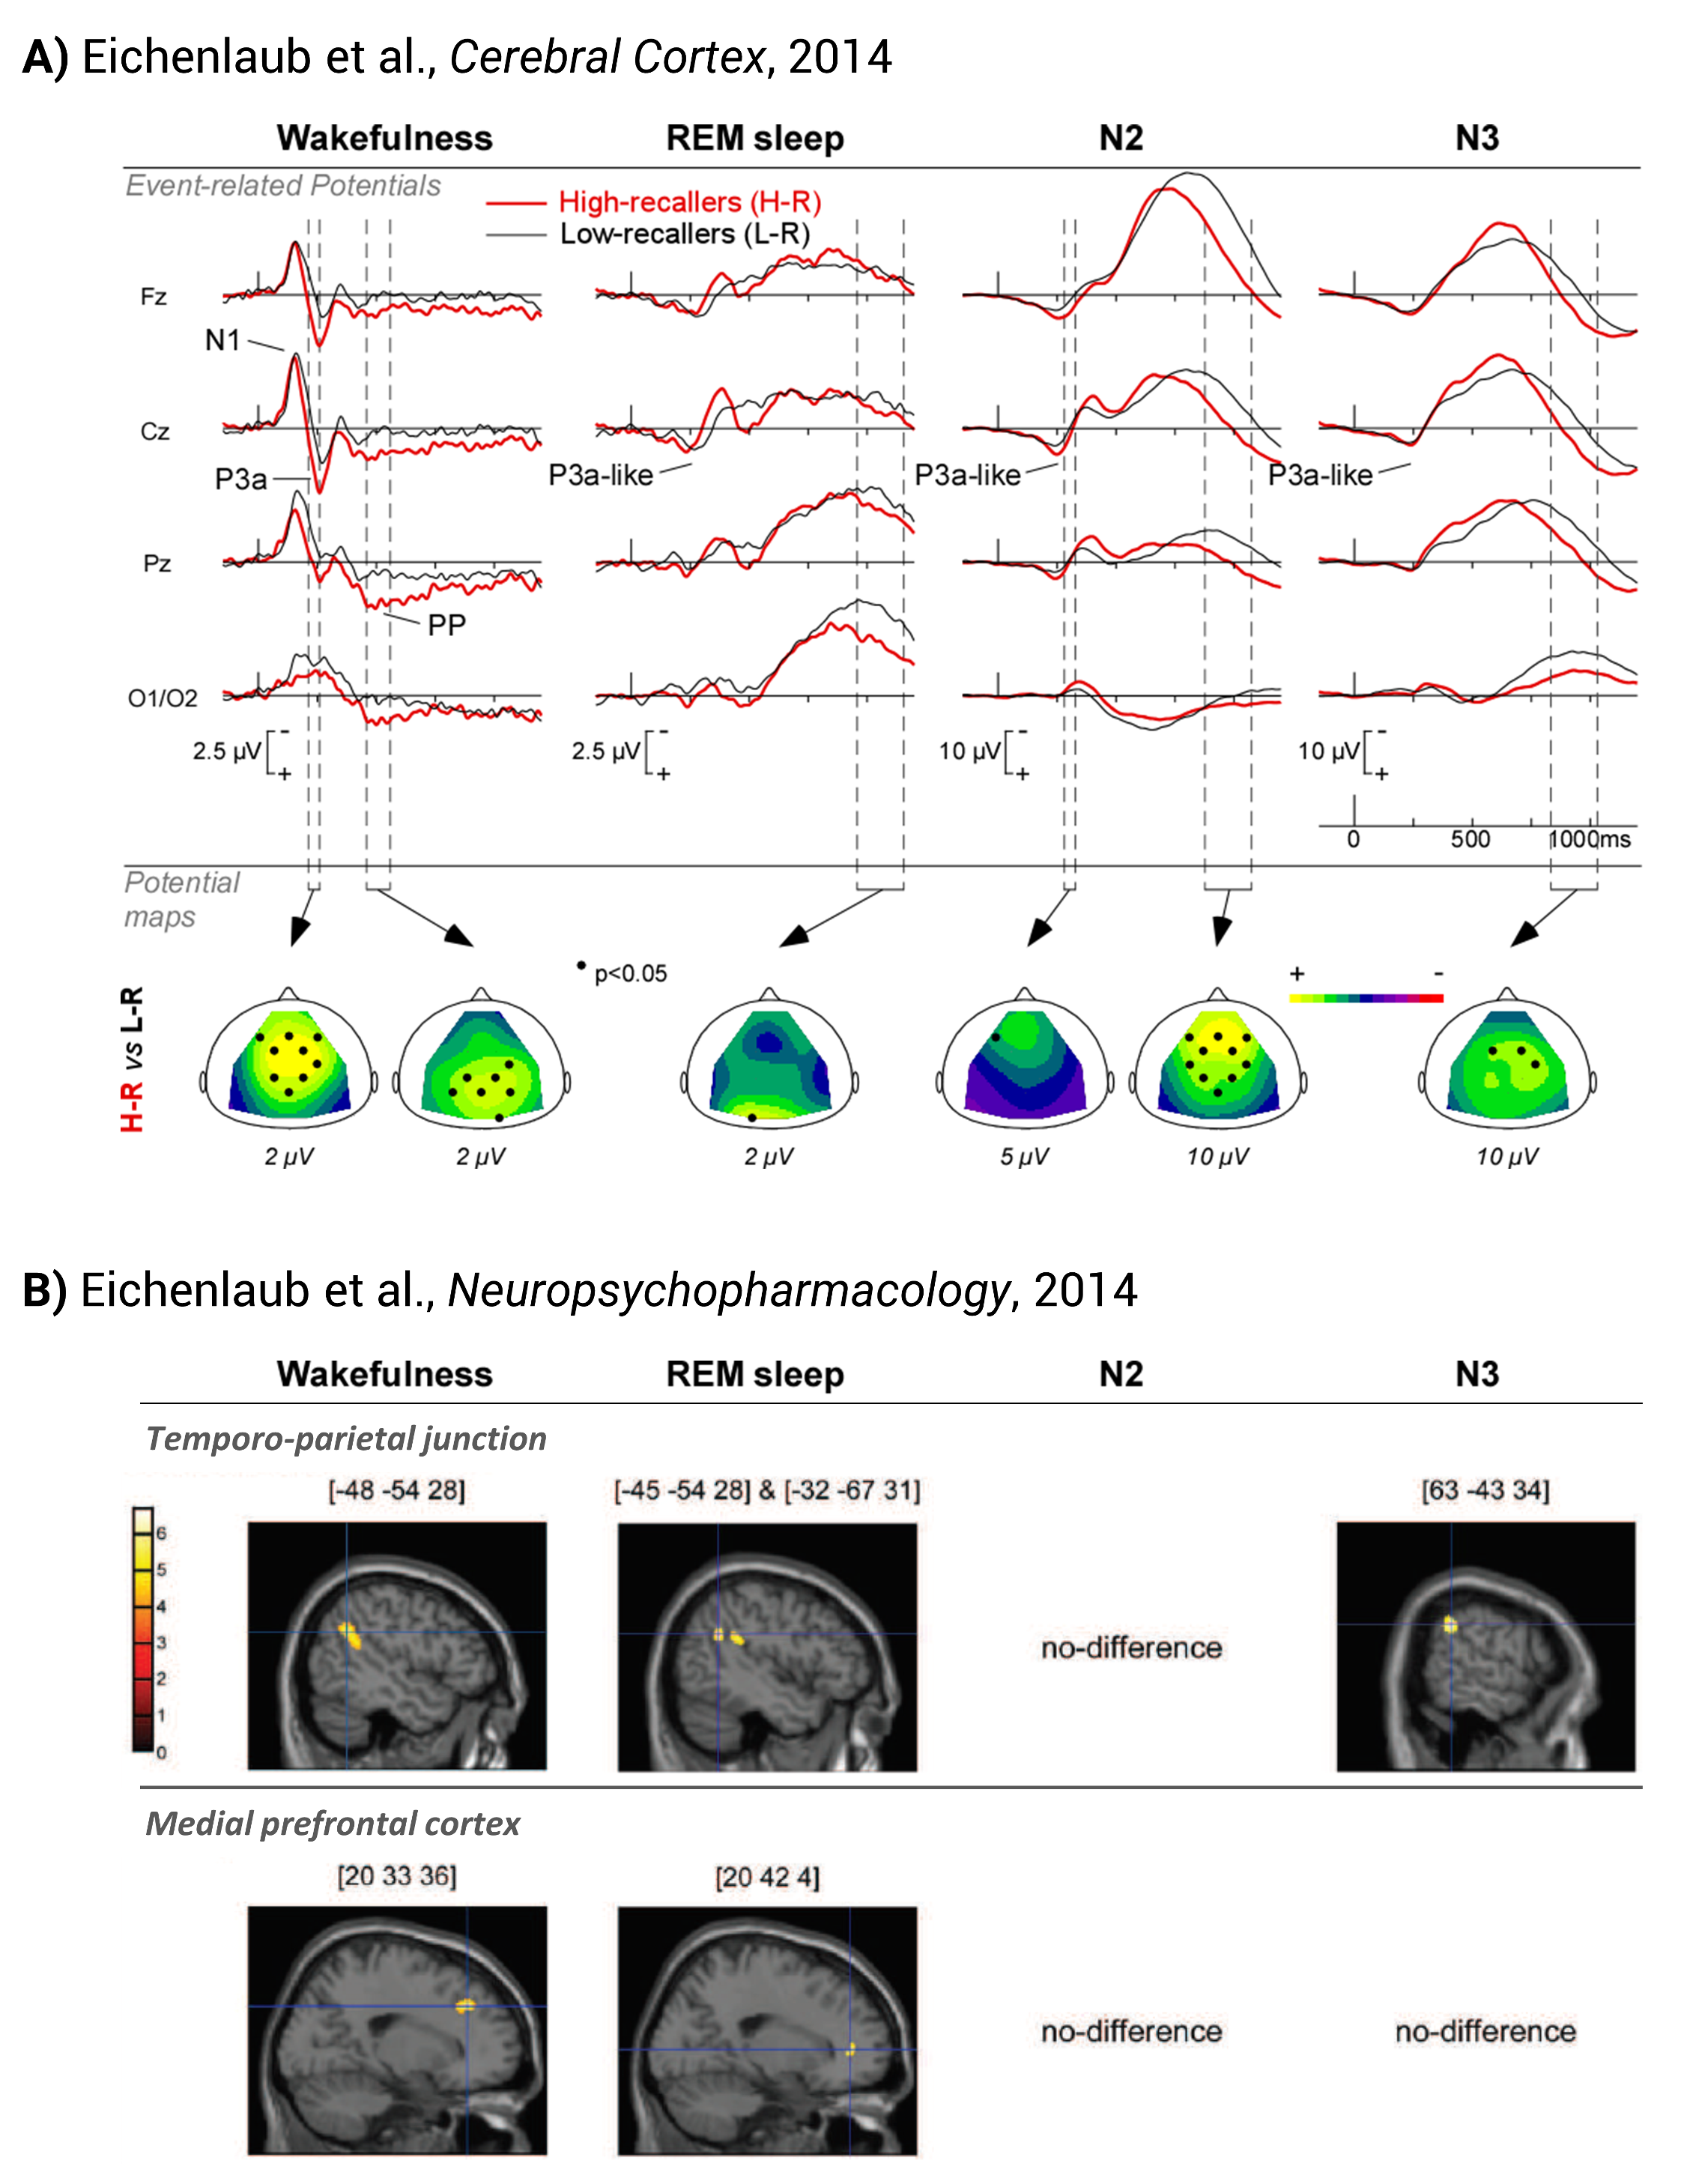
\includegraphics[width=\textwidth]{Fig/Intro/Intro_JBE_summary/Intro_JBE_summary.png}
	\caption[Summary of the results obtained in Eichenlaub's PhD thesis]{\textbf{Summary of the results obtained in Eichenlaub's PhD thesis.} \emph{Top}. EEG study. Compared to LR, HR showed larger brain responses to auditory stimuli (first names) during wakefulness, REM sleep, N2 sleep and N3 sleep. \emph{Bottom}. PET study. Compared to LR, HR showed increased spontaneous rCBF in the TPJ during wakefulness, REM sleep and N3 sleep, and in the MPFC during wakefulness and REM sleep. Altogether, these findings show spontaneous and evoked brain activity of HR and LR differ during both wakefulness and sleep, thus suggesting that DRF is associated with a specific brain functional organization.}
	\label{fig:intro:jbe-summary}
\end{figure}

\subsection{Link between neurophysiological and psychological traits}
\label{sec:dream-recall:param:link}

In conclusion, we have seen that many parameters covary with DRF. The ability to recall dreams seems to be associated with psychological and personality factors on one hand, and neurophysiological trait factors on the other hand. These results should be regarded as complementary. For instance, the fact that HRs demonstrate higher rCBF during sleep and wakefulness in the TPJ and MPFC, two regions of the DMN, is consistent with the DMN hypothesis of dreaming, and is well in line with the finding that HRs are more often absorbed in their inner worlds (i.e. day-dreaming, fantasy) and more anxious. Indeed, studies have reported a positive correlation between the activity of the MPFC during wakefulness and scores of openness to experience \citep{sutin_sex_2009} and neuroticism \citep{zald_brain_2002}.

\section{Theories on dream recall}
\label{sec:dream-recall:theories}

This section summarizes the main theories to explain variability in DRF (see also \citealp{schredl_dream_1996}).

\subsection{Freud’s repression hypothesis}
\label{sec:dream-recall:theories:freud}

Freud believed that the function of dreams is to preserve sleep by representing as fulfilled wishes that would otherwise awaken the dreamer. According to him, \q{the forgetting of the dream is in a large measure the work of the resistance} \citep{freud_interpretation_1900}, which means that dreams that are not sufficiently disguised to pass the censor will be entirely repressed and therefore forgotten. However, as highlighted by \citet{schredl_dream_1999}, it is currently impossible to test this hypothesis because we cannot access the non-recalled dreams in order to compare them to the recalled ones.

\subsection{Life-style hypothesis}
\label{sec:dream-recall:theories:life-style}

Schonbar was one of the first to investigate the psychological correlates of differential DRF. She proposed that DRF can be better explained as part of a general life-style and personality traits \citep{schonbar_differential_1965}. According to her work, high dream recallers are characterized by an ‘inner-acceptant’ life-style, which involves higher creativity, introspection, fantasy proneness and openness to experience. This hypothesis has been corroborated by several experimental studies that reported a positive association between DRF on one hand and openness to experience, absorption and creativity on the other hand (see section \ref{sec:dream-recall:param:link}).

\subsection{Salience hypothesis}
\label{sec:dream-recall:theories:salience}

Based on the idea that the principles of waking memory apply to dream recall, Cohen developed in the seventies the interference hypothesis \citep{cohen_dream_1973} followed by the salience hypothesis \citep{cohen_test_1974}. The interference hypothesis postulates that the dream memory trace remains so long as there is no distraction or interference. Otherwise, dreams are forgotten in order to maximize the memory capacity for the day ahead. This echoes French philosopher Roger Caillois’s idea on dream forgetting: \q{Dreams are quickly forgotten because they have no consequences on waking life and there is only benefits in forgetting them} \citep{caillois_incertitude_1956}. In more practical terms, the central idea of this theory is that the dreamer must voluntary pay attention to the dream immediately after awakening. In this respect, it overlaps the life-style hypothesis since high dream recallers are expected to be more interested in their dreams and therefore put more attention on them upon awakening.
Cohen further extended his model in the salience hypothesis, which states that the more salient a dream (e.g. a vivid, bizarre, and highly emotional dream content), and the less interferences there are during the recall process, the more likely the dream is to be recalled. Several findings are in favor of this hypothesis. For example, it has been shown that bizarreness \citep{cipolli_bizarreness_1993} and emotionality \citep{schredl_emotions_1998} enhance recall of dream content (an observation that was however not replicated when taking the effect of dream length into account; \citealp{schredl_relationship_2000}). More recently, \citet{parke_re-examination_2009} have studied the combined effect of interference and salience processes on dream recall. The findings suggest that a link is present, as the more interference experienced has tended to reduce the length of the dream recall in turn reducing the reported salience.

\subsection{Arousal-retrieval model}
\label{sec:dream-recall:theories:arousal}

\citet{koulack_dream_1976} proposed in their so-called arousal-retrieval model that a short period of wakefulness (arousal\footnote{\citet{koulack_dream_1976} used the word \emph{arousal} to describe a short period of wakefulness, without explicitly mentioning a minimum and maximum duration. To avoid ambiguity, it should be noted that the word \emph{arousal}, as it is used in the present thesis, refers to short events (typically 3 to 15 seconds) that are scored independently of the sleep stages and are therefore different from full (> 15 sec) awakenings; for more details see \ref{sec:problematic:arousals}}) must occur immediately after dreaming in order to transfer the dream content from short-term memory to long term memory. Furthermore, they drew on Cohen’s work to propose that the salience of dream content and lack of interferences during the recall process were critical for a successful recall of the stored dream (retrieval). The arousal-retrieval model is one of the most comprehensive model of dream recall and has received great support from the literature, reviewed earlier in section \ref{sec:dream-recall:param:sleep}.

\subsection{State-shift hypothesis}
\label{sec:dream-recall:theories:state}

Extending these arousal-based ideas, \citet{koukkou_dreaming:_1983} proposed the state-shift hypothesis which emphasizes the state dependent effects of dream recall rather than short-term memory effects. According to them, \q{forgetting of dreams is a function of the magnitude of the difference between states during encoding and recall} \citep{koukkou_dreaming:_1983}. Consequently, the closer two functional states are, the better is the transference of information. Thus, according to them, dreams are better recalled when the awake functional state
is similar to the sleeping functional state. It was argued that such compatibility occurs between wakefulness and REM sleep, enabling better recall of REM dreams. By contrast, the slow EEG frequencies of NREM sleep (and especially N3 sleep) are functionally very different from wakefulness, and this could account for the poorer NREM dream recall.

\subsection{Sleep inertia}
\label{sec:dream-recall:theories:inertia}

\citet{conduit_poor_2004} demonstrated that the cognitive performance during or shortly after awakening is of importance for the process of dream recall. The design of their study is as follows. Participants were instructed to produce an eye movement signal whenever they heard a tone, presented at increasing volume during N2 and REM sleep until an eye movement signal verification was observed.  Ninety seconds after signal verification, participants were awakened and asked if they remembered hearing the tone or responding with the EM signal. Such recollection of signal verified tone presentations was significantly less after Stage 2 sleep (65\%) compared to REM sleep (100\%) presentations. Furthermore, signal verified tone recall was significantly correlated with reported dream recall frequency. They concluded that \q{quite possibly, brain functioning underlying the reporting and non-reporting of dreams does not exist within the pre-sleeping period at all, but within the period just after awakening, when cognitive resources are in demand to recall and/or consolidate events which have just occurred within the previous sleeping period} \citep{conduit_poor_2004}.
Echoing these findings, \citet{schredl_factors_2003} noted that cognitive functioning in the period just after awakening is often severely impaired (an effect referred to as sleep inertia; \citealp{tassi_sleep_2000, trotti_waking_2016}), and that it would be in consequence \q{promising to correlate inter-individual differences regarding the sleep inertia with DRF}. This issue will form a large part of the doctoral work hereby presented and we will return to this in section \ref{sec:problematic:inertia}.

\subsection{Towards a unifying theory of dream recall}
\label{sec:dream-recall:theories:unifying}

This brief overview leads to the observation that there is a broad spectrum of dream recall theories, ranging from relating to the content of the dream (Freud’s repression and Cohen’s salience hypotheses) to accounting for the psychological (life-style hypothesis), cognitive and physiological processes (arousal-retrieval,  state-shift hypothesis, sleep inertia; see Figure \ref{fig:intro:dream-recall-models}). The empirical data seems hitherto to fit best into the arousal-retrieval model (which integrates elements of both the Salience and Interference hypotheses) and the life-style hypothesis. A comprehensive, unified theory of dream recall should combine these two models, for example using the arousal-retrieval model to account for day-to-day variability in DRF (state factors), and the life-style hypothesis to account for the large inter-individual DRF variability (traits factors). Moreover, there is a currently a lack of evidence for the state-shift hypothesis (due to the difficulty of deriving valid quantitative measures for the closeness of functional states; \citealp{schredl_dream_1999}) and the sleep inertia theory, which both insist on brain functioning within the period just after awakening.

\begin{figure}[!htb]
	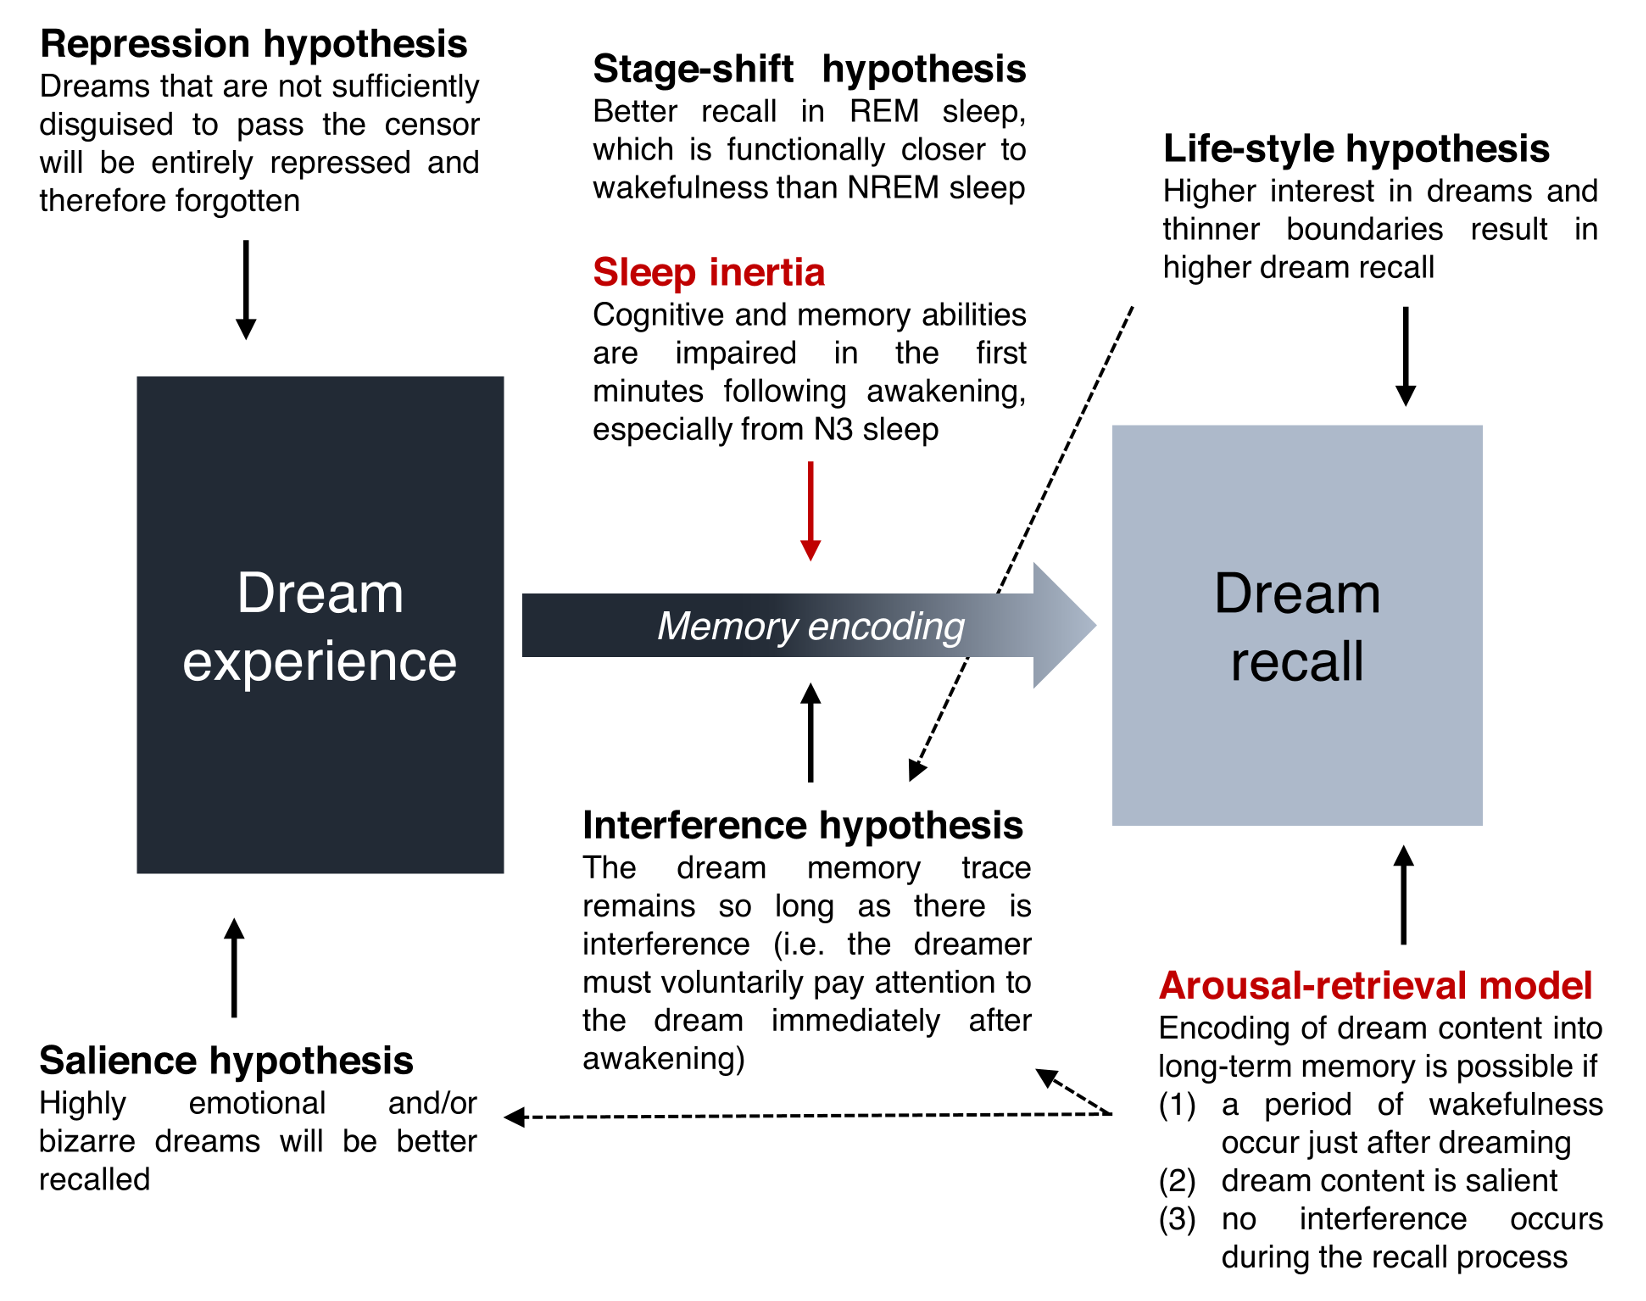
\includegraphics[width=\textwidth]{Fig/Intro/Intro_DRF_model/Intro_DRF_model.png}
	\caption[Dream recall theories]{\textbf{Dream recall theories.} The arousal-retrieval model provides so far the most comprehensive theory on dream recall and is firmly grounded in empirical evidence. At its simplest, it states that a short period of wakefulness must occur just after dreaming (arousal) in order to transfer the dream content from short to long term memory, which is otherwise impossible during sleep. In addition, it postulates that the dream content must be salient (Salience hypothesis, e.g. highly emotional, vivid and/or bizarre) and that the dreamer must voluntarily pay attention to the dream content (Interference hypothesis). Notably, it is very probable that the individuals with the greatest interest in dreams (Life-style hypothesis) are also the ones which focus the more on their dreams immediately after awakening, thus reducing encoding interferences. This would provide a link between the Life-style hypothesis and the arousal-retrieval model. Finally, sleep inertia could be a important explanatory factor with regards to DRF. It is possible that low dream recallers experience more acute sleep inertia upon awakening, whatever the sleep stage before awakening. More impaired memory and cognitive abilities upon awakening would in turn prevent the encoding of dreams to long term-memory. However, this hypothesis remains to be tested empirically.}
	\label{fig:intro:dream-recall-models}
\end{figure}

\cleardoublepage
\cleardoublepage

\chapter{Dream content}
\label{sec:dream-content}

\cleanchapterquote{Prétendre donner les rêves comme de simples jeux de la pensée, de simples images de l’imagination, c’est témoigner d’un manque de réflexion ou de loyauté ; car de toute évidence ils en diffèrent spécifiquement. Les images de l’imagination sont faibles, languissantes, incomplètes, partielles et si fugitives qu’on peut à peine fixer dans sa mémoire pendant quelques secondes les traits d’un absent, et que même le jeu le plus vif de l’imagination ne peut nullement entrer en comparaison avec la réalité palpable que le rêve met sous nos yeux.}{Schopenhauer}{Parerga und Paralipomena, 1851}

\section{Basic principles of dream content analysis}
\label{sec:dream-content:method}

Empirical investigation on dreaming started in the nineteenth century when amateur researchers started to quantify aspects of their dream content. One notable example is the pioneering paper of Mary Calkins \citeyearpar{calkins_statistics_1893}, entitled \q{Statistics of dreams}, in which she reported, inter alia, statistics concerning dream length and vividness, dream characters and dream- and waking-life associations. Since then, a considerable numbers of scales and rating systems for dream content analysis have been developed \citep{schredl_dream_2010}. Most of them are based on automatic analysis of the lexical content of dream reports, a method which has the advantages of minimizing the experimenter bias and being replicable by other research groups. Perhaps the most famous is the Hall \& Van de Castle system, which have provided a global profile of dream content dimensions in young adult \citep{hall_content_1966}. It remains today the major reference since it has proven stable over at least one generation \citep{hall_dreams_1982}.

\section{Quantitative results}
\label{sec:dream-content:quant}

Results from several decades of dream content studies \citep{hall_content_1966, schwartz_exploration_1999, schredl_characteristics_2010} indicate that: dreams tend to be negative on many dimensions and aggressions are more frequent than friendly interactions, visual imagery occurs more frequently in dreams than imagery of other senses (audition, olfaction, touch, and taste); the dream drama is mostly lived by the dreamer from a first-person perspective; some elements of real-life events previously experienced by the dreamer often contribute to the scene of the dream; most often, the dream sequence is not within the dreamer’s voluntary control (i.e., the dreamer may be convinced during the dream that the dream’s story is really happening); temporal and spatial incoherencies can occur in the dream story; the dream report is often full of people interacting with each other (e.g., discussions, fights, pursuit, sexuality); and finally, the dream report often contains strong emotions.
Gender differences in dream content have been consistently reported. For example, men report more often physical aggression and sex than women \citep{nielsen_typical_2003, schredl_typical_2004}.
Finally, many aspects of the subject’s daily life influence dream content (reviewed in \citealp{ruby_experimental_2011}), including news event, musical practice, current concerns and religious beliefs, chronic pain, mood or living in a violent environment.

\section{The sources of dream content}
\label{sec:dream-content:sources}

Based on these experimental findings, \citet{de_koninck_sleep_2012} has reviewed in his book entitled \q{Sleep, dreams and dreaming} the sources that mediate dream construction, as well as their relative contribution to the dream content. He proposed that the different sources of dreams are best represented in a pyramidal manner, from low, more biological levels, predominant in shaping the dream content, to higher, more cognitive levels, that carry much less influence to the dream content (Figure \ref{fig:intro:koninck}).

\begin{figure}[htb]
	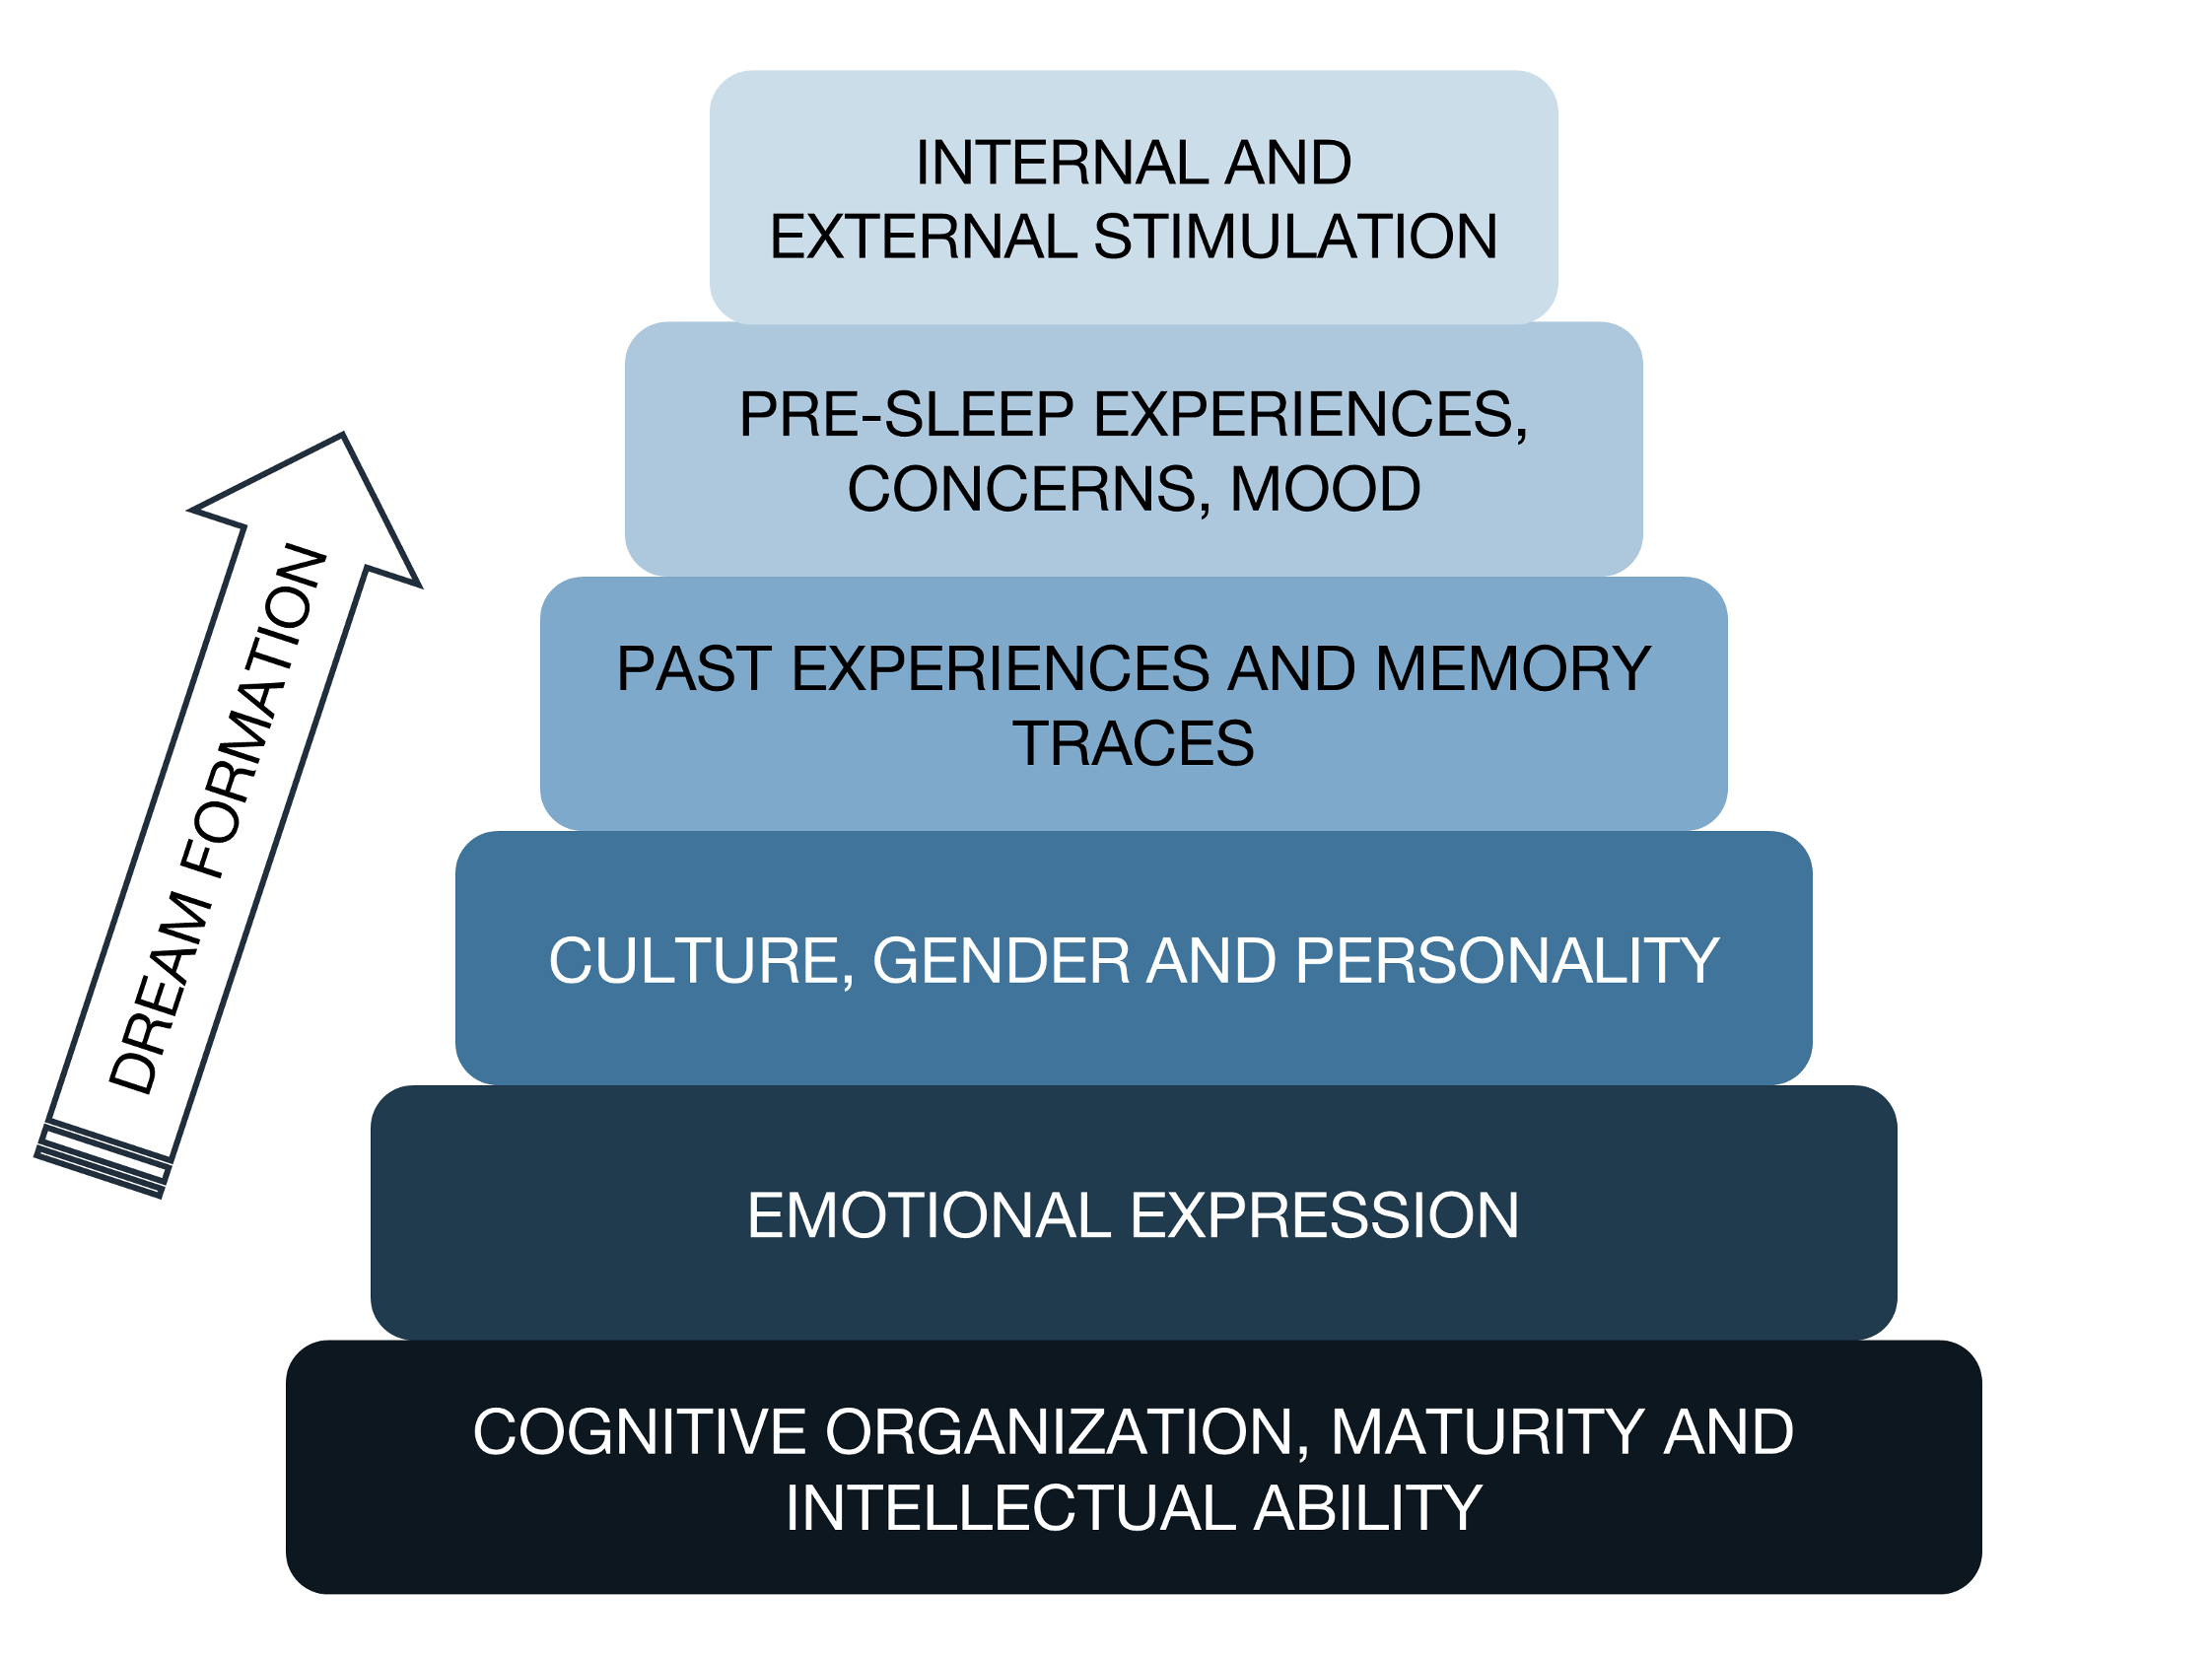
\includegraphics[width=\textwidth]{Fig/Intro/Intro_Pyramid_dream_construction/Intro_pyramid_dream.png}
	\caption[Layers in the construction of dreams]{Layers in the construction of dreams \citep{de_koninck_sleep_2012}. The various factors in the elaboration of dreaming are illustrated as a pyramid suggesting their order and importance.}
	\label{fig:intro:koninck}
\end{figure}

\subsection{The memory sources of dream content}
\label{sec:dream-content:sources:memory}

As we mentioned earlier, there is ample evidence that waking experience finds its way into dreams. However, the characteristics and time course of the waking memory sources integrated into dreams are still unclear. For instance, it is now clear that dream content very rarely replays an episodic memory as it is remembered \citep{fosse_dreaming_2003, nielsen_what_2005}, although it is often related to some elements of the waking life of the dreamer \citep{schredl_characteristics_2010, blagrove_trait_2010, ruby_experimental_2011}. This observation has led to the so-called \q{continuity hypothesis of dreaming} which simply states that dreams reflect waking life experiences \citep{schredl_continuity_2003}.

Several factors have been positively associated with the likelihood of a waking life experience to be incorporated into dreams \citep{schredl_characteristics_2010}. These factors are reviewed in the following lines. First, there seems to be a linear decrease in temporal references identified in dreams, with recent experiences being more incorporated into dreams than older ones \citep{botman_dream_1990, strauch_dem_2004, grenier_temporal_2005}. This finding supports the notion of continuity between waking and dreaming memory processes. Furthermore, several studies \citep{botman_dream_1990, nielsen_day-residue_1992, marquardt_empirical_1996} have confirmed that a significant proportion of dreams contain elements that refer to experiences of the preceding day, a phenomenon known as day-residues and mentioned by Freud who considered them as \q{a necessary ingredient in dream formation} \citep{freud_interpretation_1900}. Another interesting finding is that contrary to what would be expected according to memory decay with time, some studies reported an overrepresentation in dreams of waking experiences that happened approximately one week before the dream \citep{nielsen_day-residue_1992, marquardt_empirical_1996}, however this effect was found only for REM dreams and not N2 or N3 dreams \citep{blagrove_assessing_2011, van_rijn_dream-lag_2015}. Second, there is a preferential incorporation of emotional waking-life experiences into dreams \citep{malinowski_evidence_2014, schredl_factors_2006}. Interestingly, emotional intensity, but not emotional tone seems to affect the incorporation into subsequent dreams. Third, all waking life activities are not represented in the same proportion in dreams \citep{hartmann_we_1996, schredl_continuity_2000}. Focused thinking activity (such as using a computer, reading) are rarely reported in dreams, an effect that may be explained by the generally low emotional intensity of these types of activities. Fourth, the magnitude of the continuity between waking and dreaming is related to some extent to the personality traits of the dreamer \citep{schredl_dreaming_1996}. Finally, chronobiological factors, such as sleep cycles and time of the night, influence dream content. For example, dream reports from the first part of the night comprise more elements of the previous day than dream reports from the second part of the night \citep{roffwarg_effects_1978}.


\cleardoublepage
\part{METHODS}
%% !TEX root = ../thesis-example.tex
%
\chapter{Related Work}
\label{sec:related}

\cleanchapterquote{A picture is worth a thousand words. An interface is worth a thousand pictures.}{Ben Shneiderman}{(Professor for Computer Science)}

\Blindtext[2][1]

\section{Related Work Section 1}
\label{sec:related:sec1}

\Blindtext[2][2]

\section{Related Work Section 2}
\label{sec:related:sec2}

\Blindtext[3][2]

\section{Related Work Section 3}
\label{sec:related:sec3}

\Blindtext[4][2]

\section{Conclusion}
\label{sec:related:conclusion}

\Blindtext[2][1]
 		% INCLUDE: related work

% 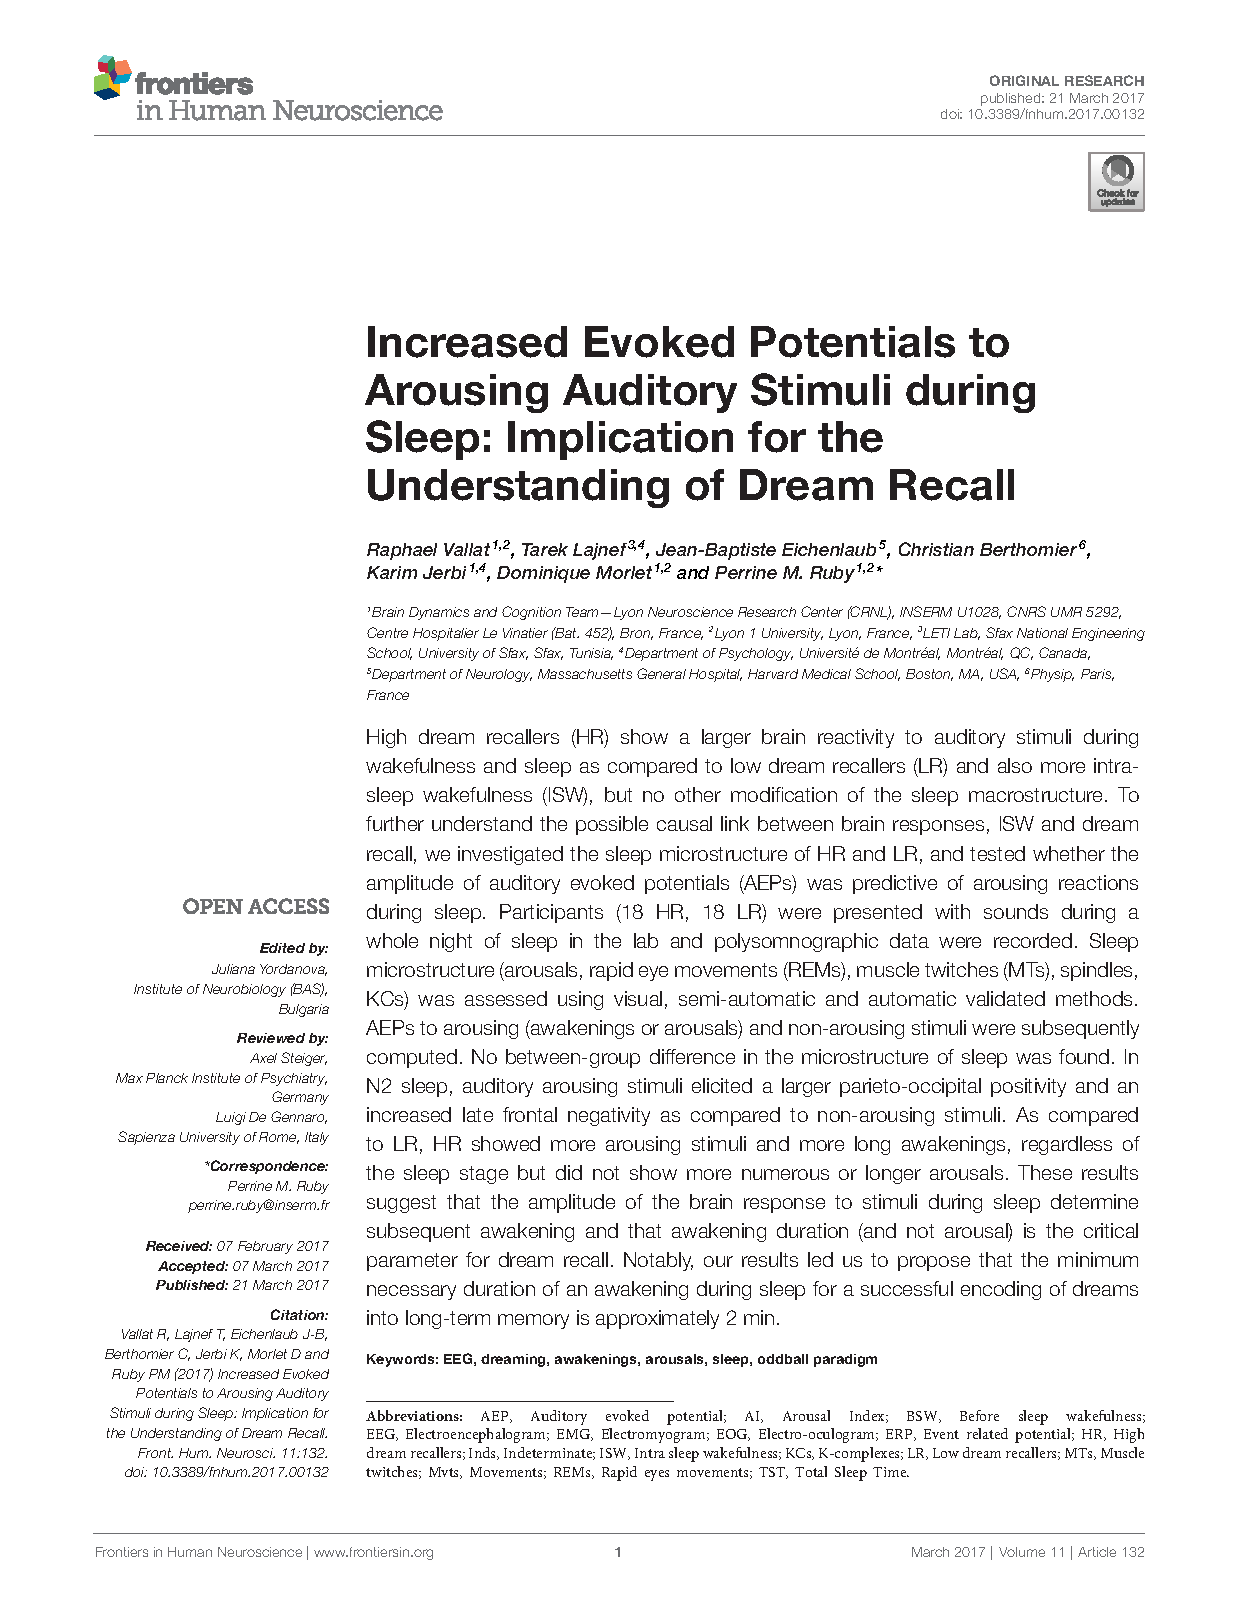
\includepdf[pages=-, pagecommand={\thispagestyle{plain}}]{article/Vallat_2017_FHN.pdf}

%% !TEX root = ../thesis-example.tex
%
\chapter{Conclusion}
\label{sec:conclusion}

\Blindtext[2][1]

\section{System Section 1}
\label{sec:conclusion:sec1}

\Blindtext[2][2]

\section{System Section 2}
\label{sec:conclusion:sec2}

\Blindtext[3][2]

\section{Future Work}
\label{sec:conclusion:future}

\Blindtext[2][2]
 			% INCLUDE: conclusion

\cleardoublepage
\part{EXPERIMENTAL RESULTS}

% --------------------------
% Back matter
% --------------------------
\cleardoublepage
\part{REFERENCES}
{%
\setstretch{1.1}
\renewcommand{\bibfont}{\normalfont\small}
\setlength{\biblabelsep}{0pt}
\setlength{\bibitemsep}{0.5\baselineskip plus 0.5\baselineskip}
\printbibliography[nottype=online]
% \printbibliography[heading=subbibliography,title={Website},type=online,prefixnumbers={@}]
}
\cleardoublepage

% \listoffigures
% \cleardoublepage
%
% \listoftables
% \cleardoublepage

% % !TEX root = ../thesis-example.tex
%
\pagestyle{empty}
\hfill
\vfill
%\pdfbookmark[0]{Colophon}{Colophon}
\section*{Colophon}

This thesis was typeset with \LaTeXe.
It uses the \textit{Clean Thesis} style developed by Ricardo Langner.
The design of the \textit{Clean Thesis} style is inspired by user guide documents from Apple Inc.

Download the \textit{Clean Thesis} style at \url{http://cleanthesis.der-ric.de/}.

% \cleardoublepage

% % !TEX root = ../thesis-example.tex
%
%************************************************
% Declaration
%************************************************
\pdfbookmark[0]{Declaration}{Declaration}
\chapter*{Declaration}
\label{sec:declaration}
\thispagestyle{empty}

You can put your declaration here, to declare that you have completed your work solely and only with the help of the references you mentioned.

\bigskip

\noindent\textit{\thesisUniversityCity, \thesisDate}

\smallskip

\begin{flushright}
	\begin{minipage}{5cm}
		\rule{\textwidth}{1pt}
		\centering\thesisName
	\end{minipage}
\end{flushright}

%*****************************************
%*****************************************

% \clearpage
% \newpage
% \mbox{}

% **************************************************
% End of Document CONTENT
% **************************************************
\end{document}
